\section{Results}


\subsection{Host Species Prediction with Machine Learning}

\gls{iav} is known to infect a wide range of hosts, with subtypes (e.g. H1N1) oftentimes prefering one species over another~\cite{Rambaut2008-pm}. We hypothesized that the distribution of an IAV genome's codon usage holds enought information to assign a sequence to its corresponding host with the sequence string as single input. IAV infects a large range of birds and mammals. For some of them, like whales or horses, only limited sequence information is present, so we restricted our investigation to the three largest host groups (where large means most archived sequences): Avian, Human and Swine.


\subsubsection{Codon Usage Can Separate Host Species}

The codon usage of \gls{iav} genomes does not show large variation accross host species (Figure \ref{fig:distribution-codon}). Genome here refers to the concatenated sequence of all 8 \gls{iav} genome fragments, the protein products of which (excluding splicing variants and frame shift products) are HA, NA, NS1 and NS2, M1 and M2, as well as the \gls{rdrp} constituted by PA, PB1 and PB2. We will from now on label the genomic sequence segments with their protein products for clarity.


\begin{sidewaysfigure}
    \centering
    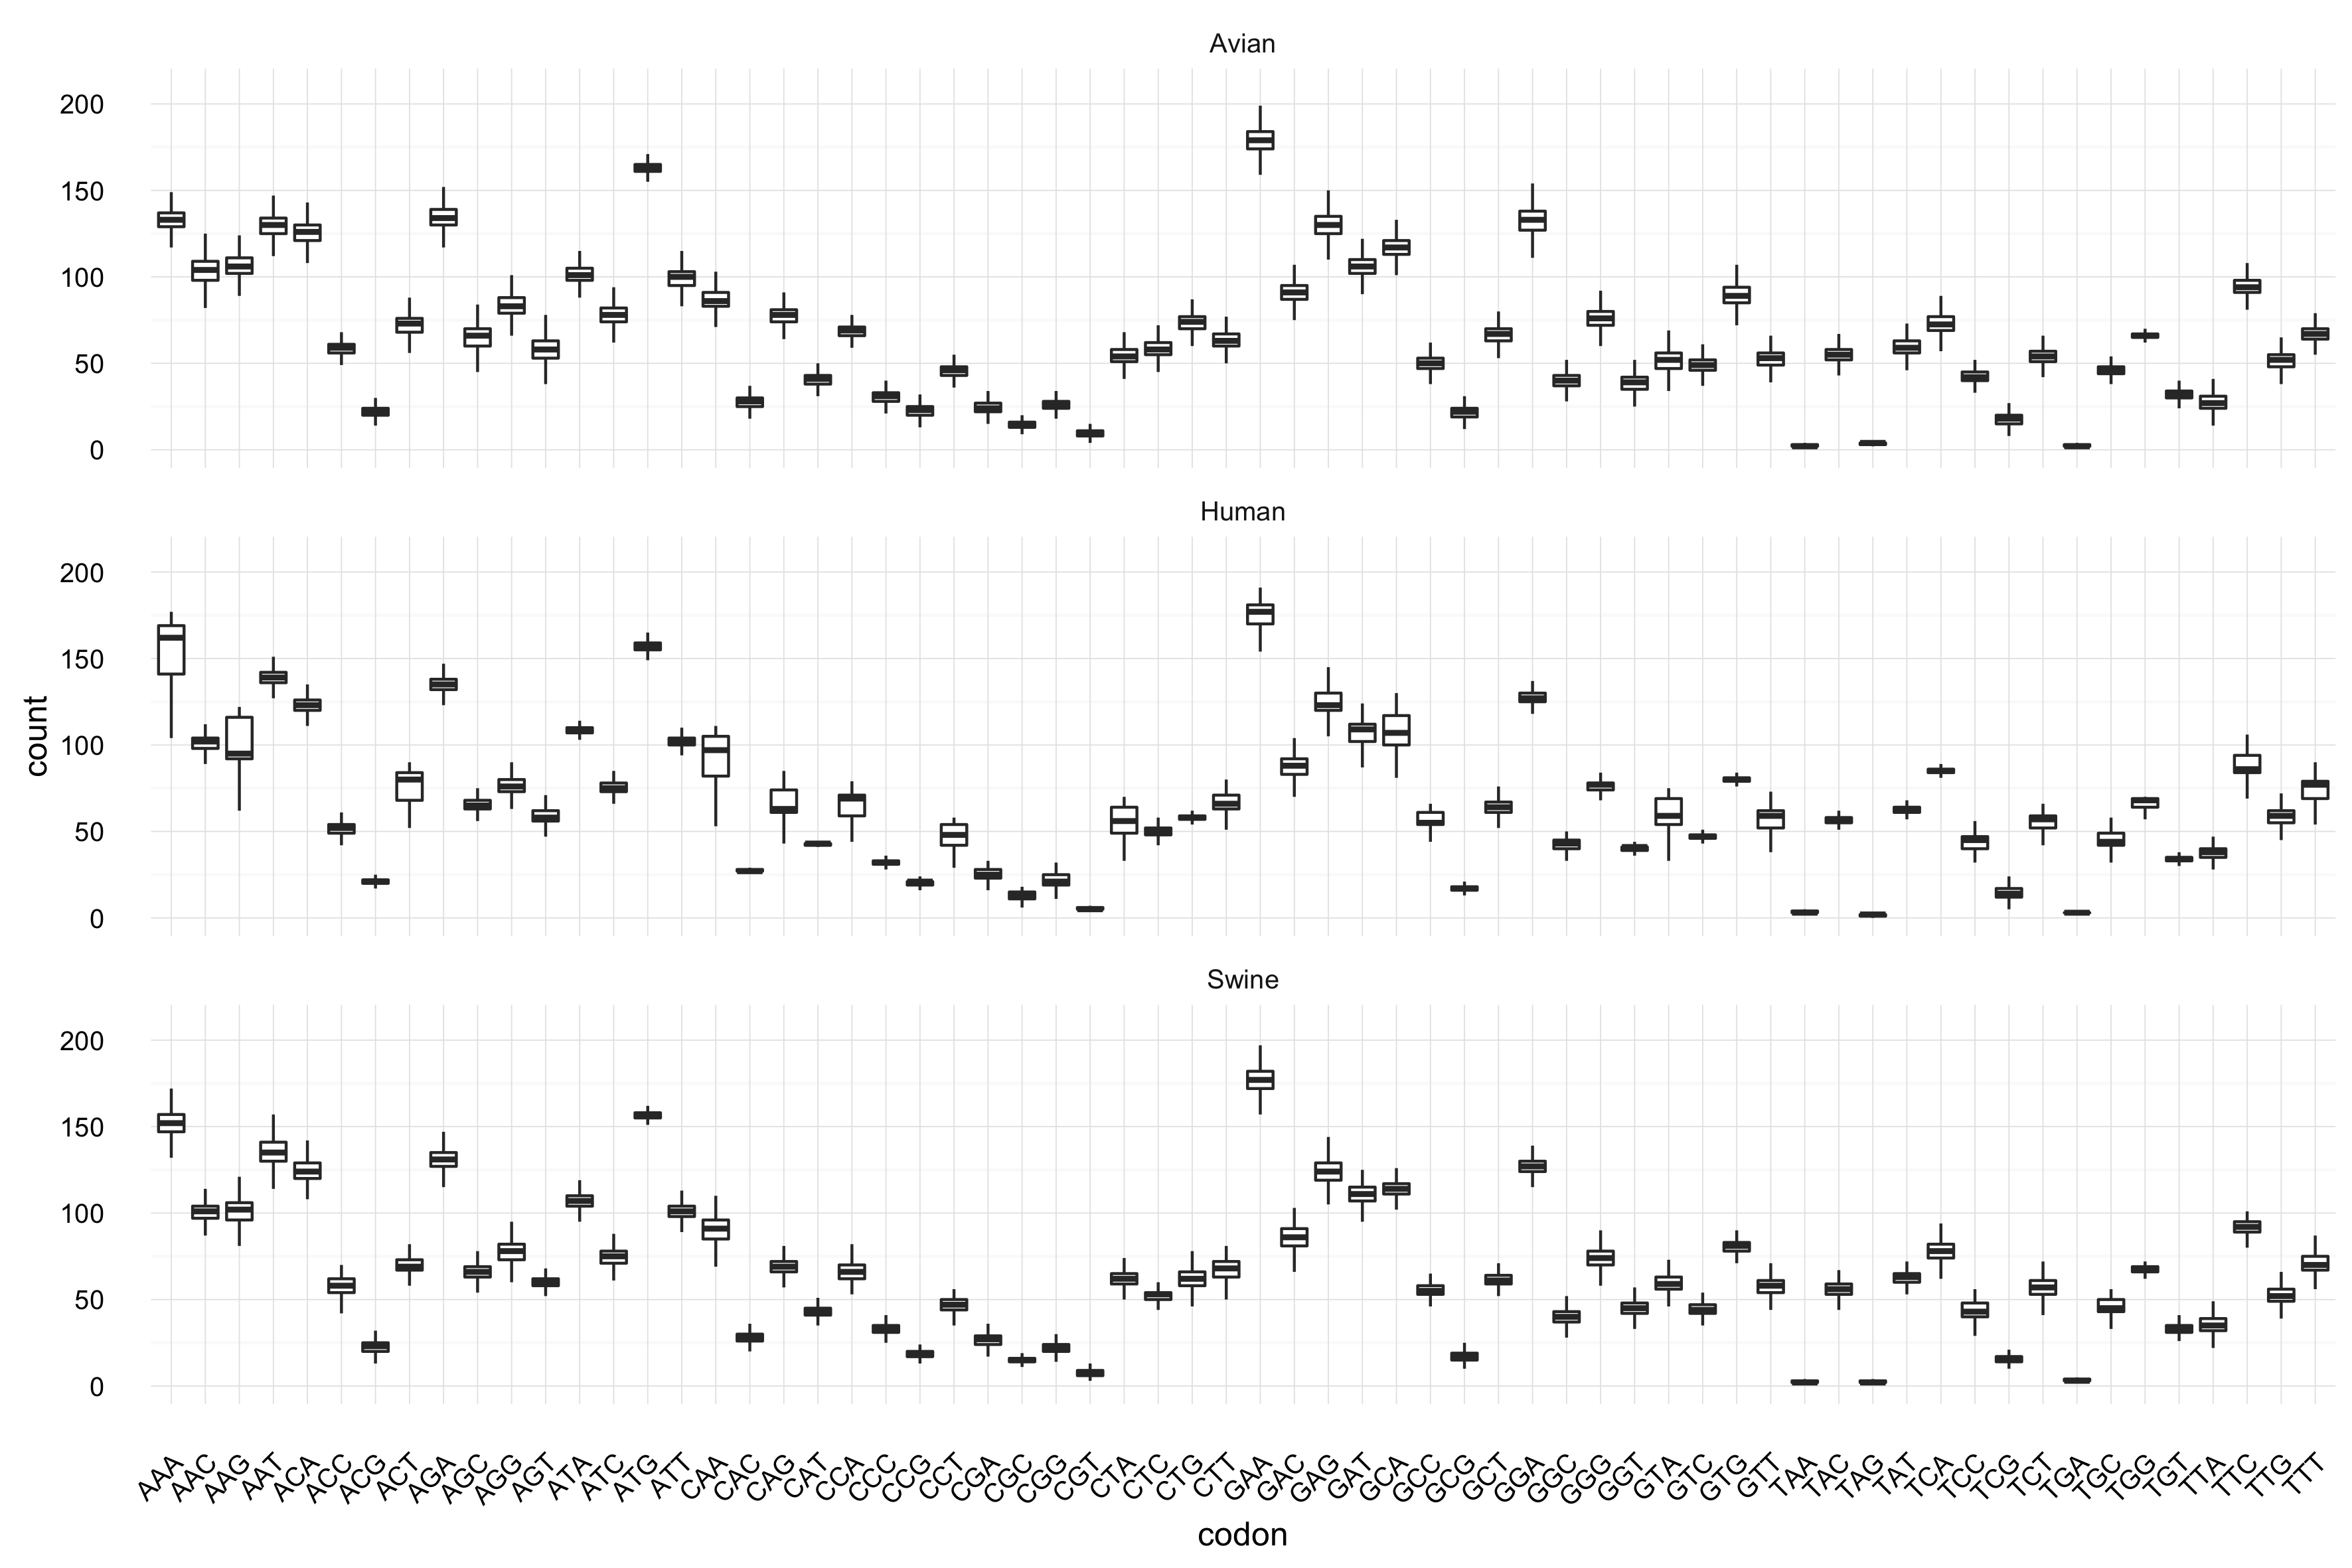
\includegraphics[scale=0.15]{boxplot_016c0.png}
    \caption[Codon usage of complete IAV genome.]{Codon usage does not show large variance accross host species (Avian, Human, Swine) as can be assessed from the boxplots accross ``columns'' in the plot facets. The x-axis displays trinucleotide combinations and the y-axis records the respective count, in aggregate referred to as codon count distribution of codon usage. Included in the analysis were 25k sequences of IAV.}
    \captionsetup{width=0.8\paperheight}
    \label{fig:distribution-codon}
\end{sidewaysfigure}


If we look at the count usage for individual segments, we can observe considerable variance between segments, but not between species (Figure \ref{fig:distribution-2nt}). We chose to plot only dinucleotides instead of codons in Figure \ref{fig:distribution-2nt} for reasons of pictorial clarity. The conclusions for di- and trinucleotides are identical. For example, comparing HA or NA to PB1, we observe a considerable drop in variance. We infer that the the nucleotide composition of segments such as PB1 is more constrained than others such as HA. One explanation is that because NA and HA are exposed to the host's immune system by being situated at the virus surface, stronger evolutionary pressures apply to mutate to escape immunity, which in turn results in greater variance of nucleotide composition. On the other end of the variance spectrum, RdRp components such as PB1 and PB2 are fundamental to virus replication and therefor more conserved.


\begin{figure}[H]
    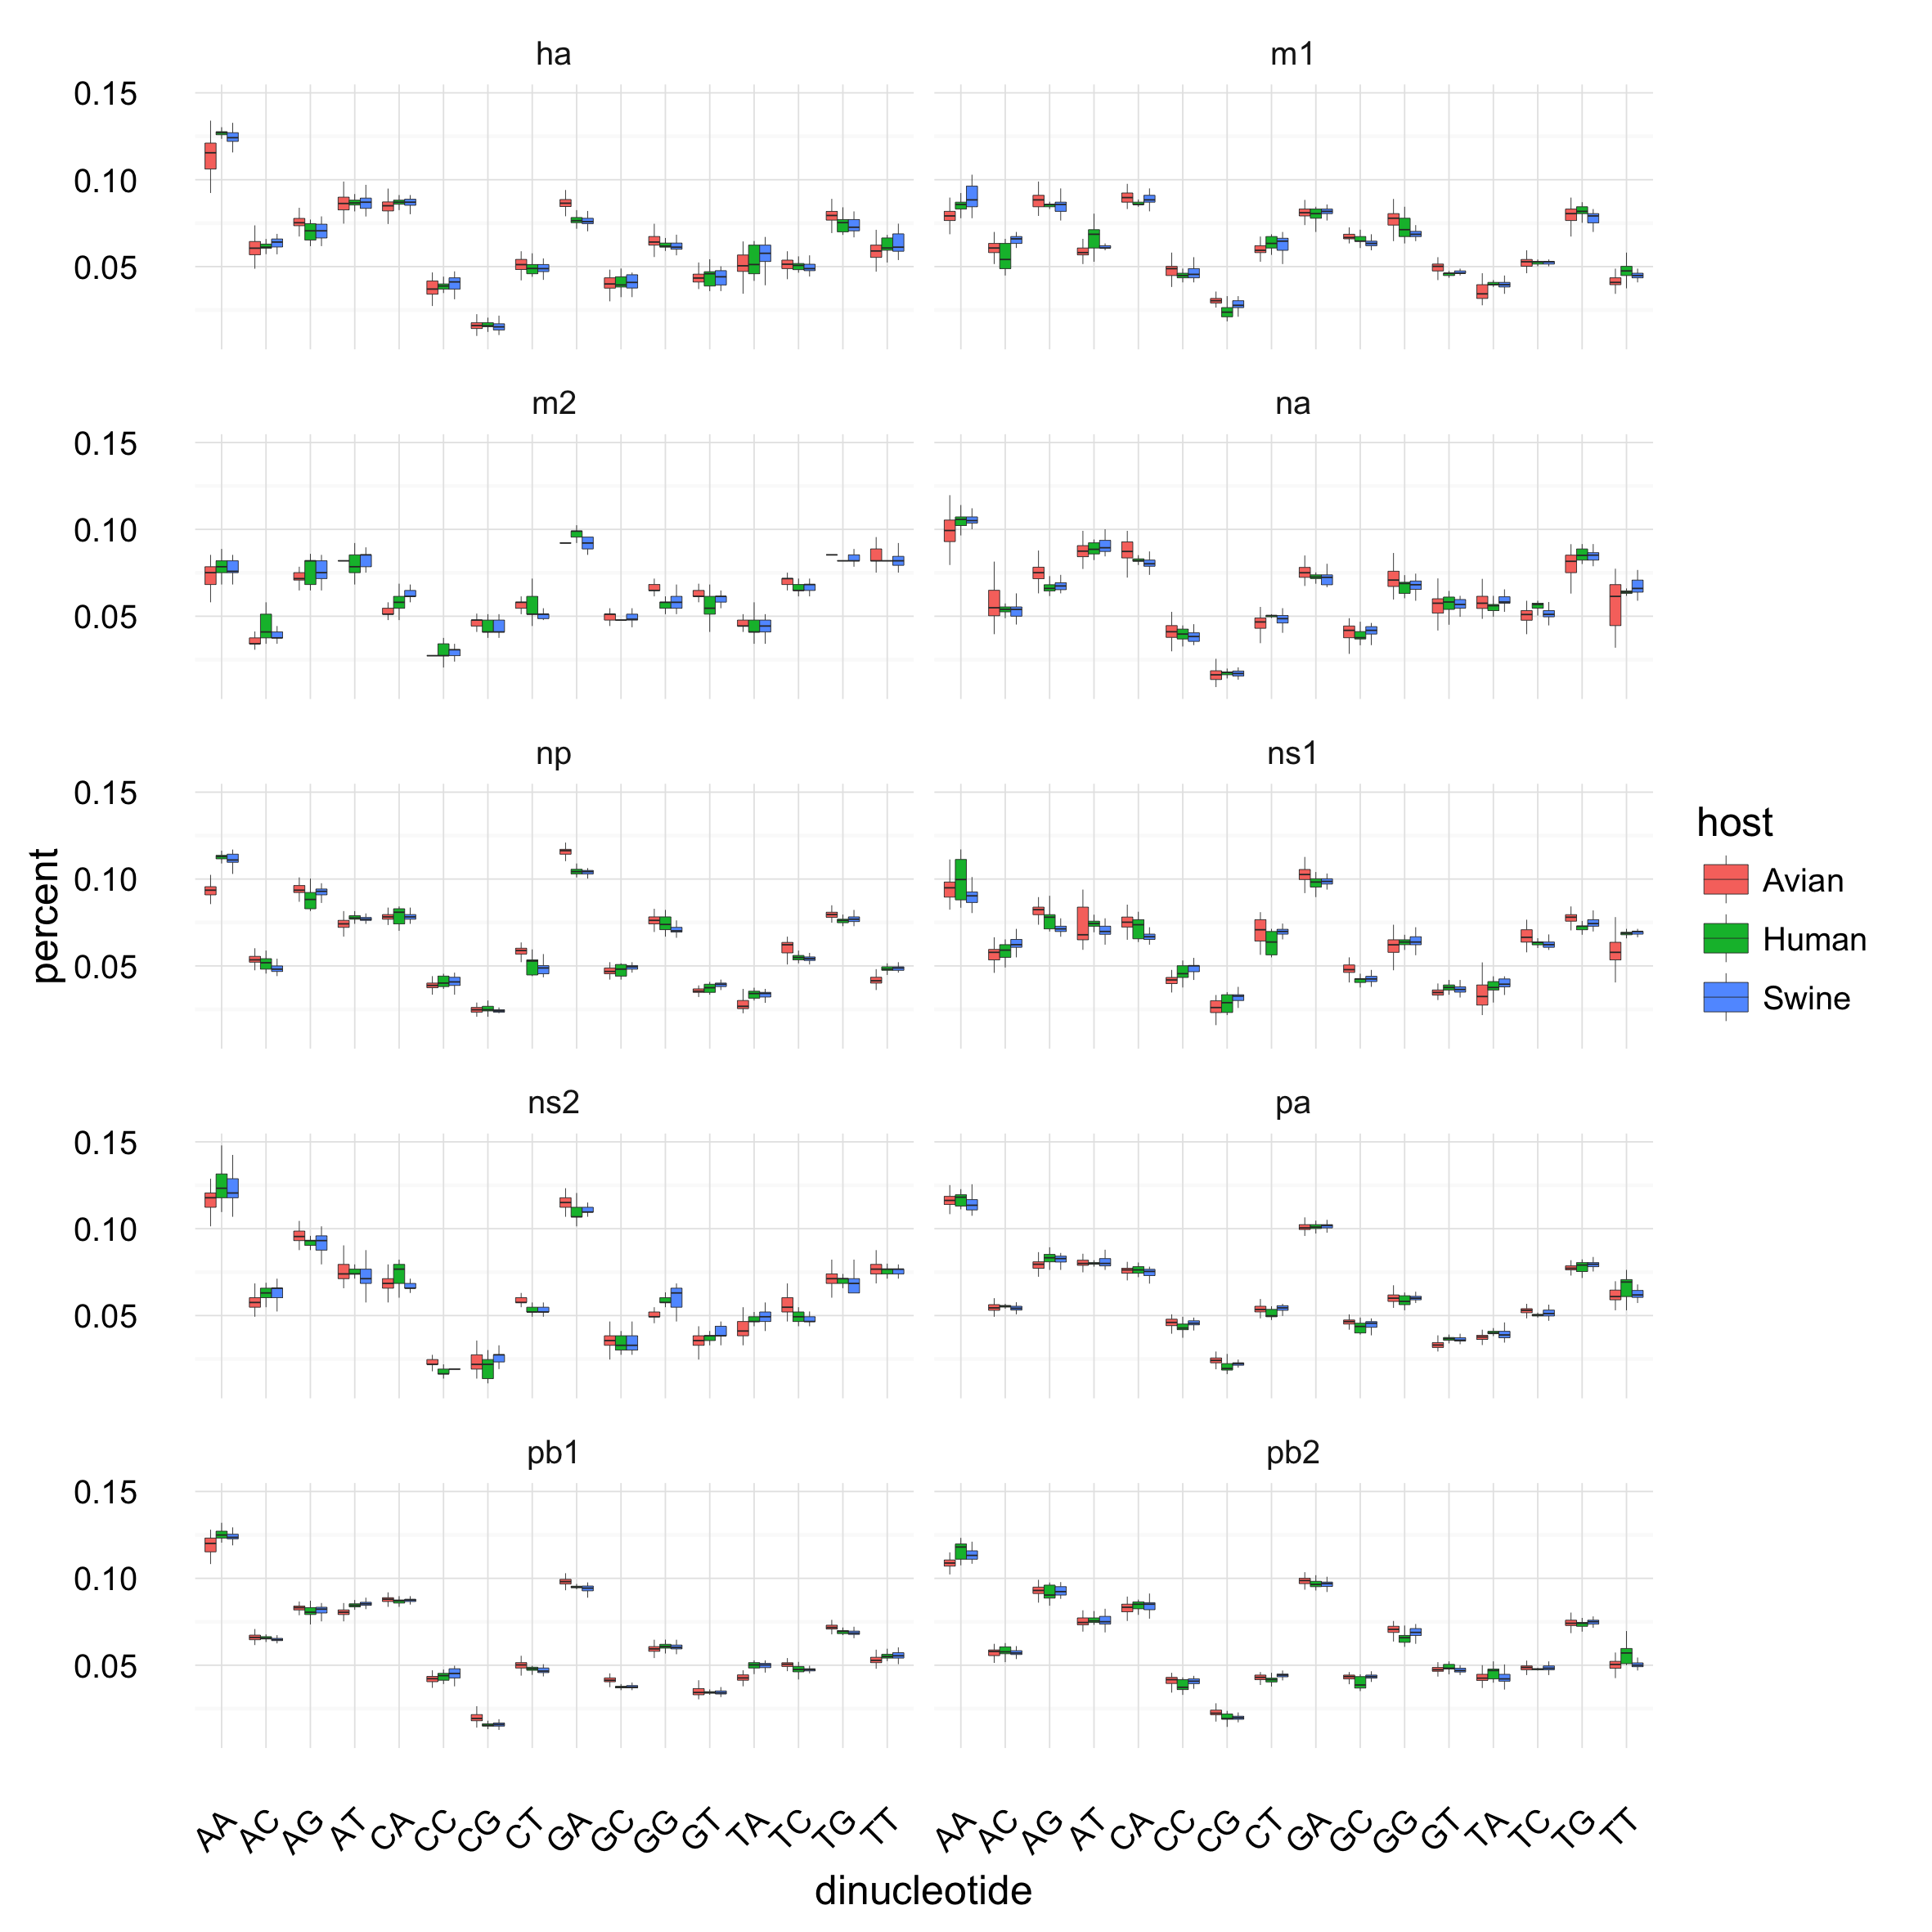
\includegraphics[scale=0.18]{kmer_2_1_segment_1d347.png}
    \caption[Dinucleotide usage of IAV genome segments.]{(Relative) dinucleotide usage differs according to IAV genome segment with plausible explanation of this observation in the different functions and constraints (see main text). Axes as in \ref{fig:distribution-codon}.}
    \label{fig:distribution-2nt}
\end{figure}


Although simply by ``eyeballing'' Figures \ref{fig:distribution-codon} and \ref{fig:distribution-2nt} one might suspect that too little variation is present to separate the sequences into distict classes. Using PCA, IAV genome samples form distinct and host-specific clusters in the first 2 principal components (Figure \ref{fig:pca1}). This means that host species can be demarcated by their (normalized) codon counts.


\begin{figure}[H]
    \begin{center}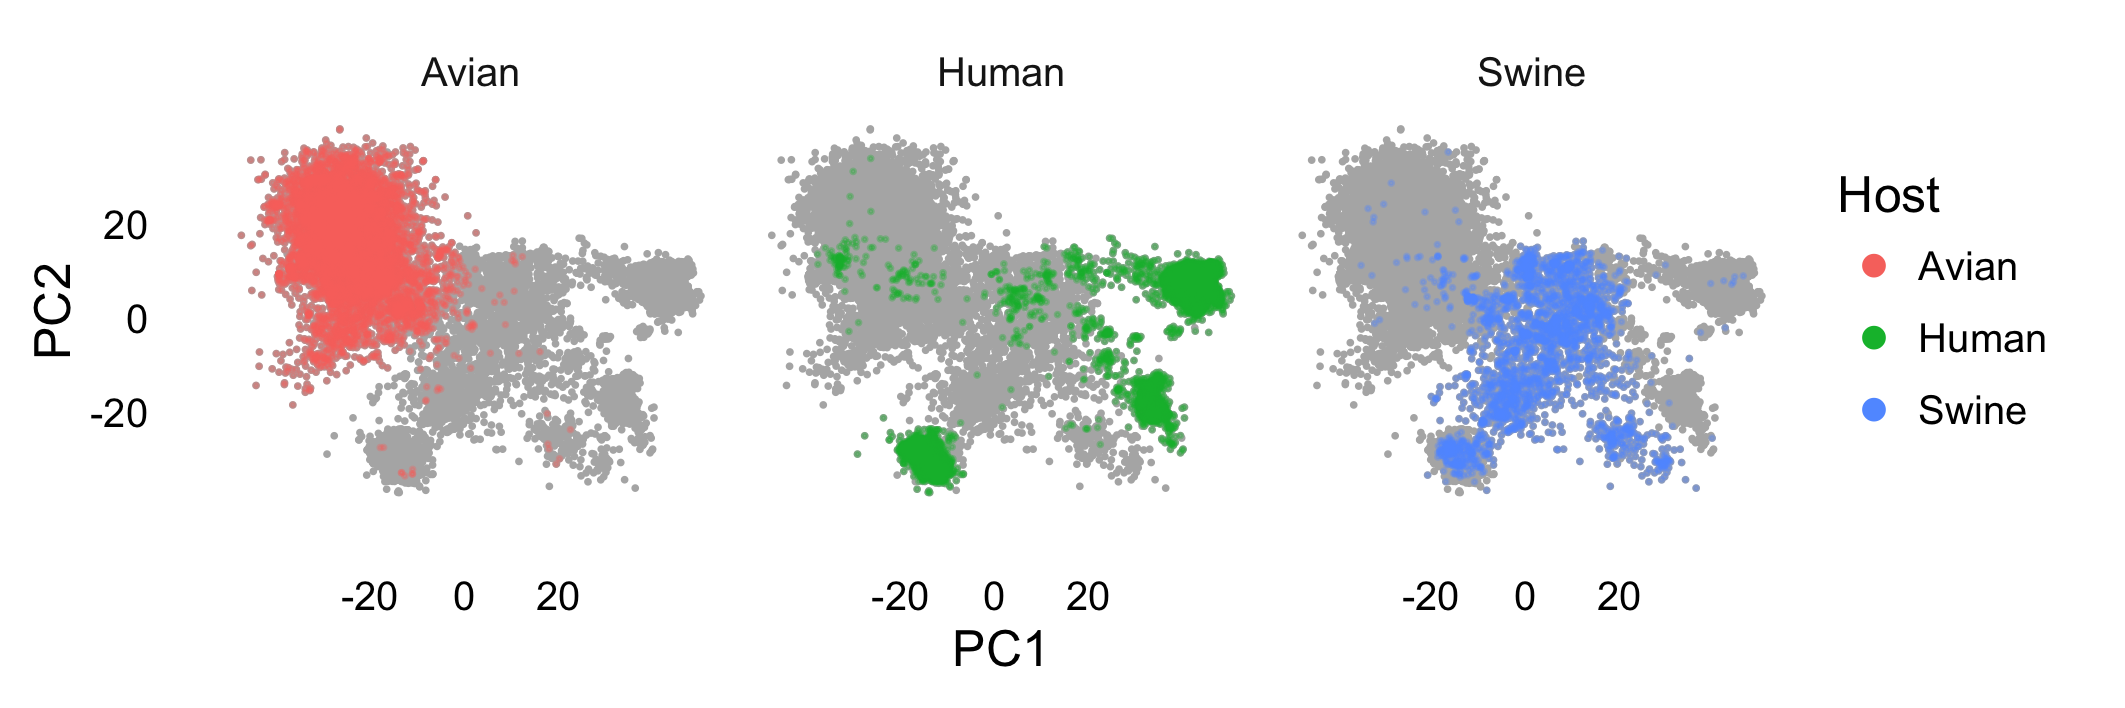
\includegraphics[scale=0.18]{pca_5b08d.png}\end{center}
    \caption[Host-specific clusters of codon usage via PCA.]{Codon usage of IAV sequences yields host-specific clusters when analysed with PCA. Principal components 1 (PC1) and 2 (PC2) are displayed (PCs are unitless). Host clusters (coloured points) have been superimposed in the respective plot facets onto the aggregate data (grey points).}
    \label{fig:pca1}
\end{figure}


More surprisingly, crudely clustering codon usage even allows the separation of various IAV subtypes. The observed clustering is hierarchical: Within ``host clusters'', IVA genome samples cluster according to their subtype (e.g. H1N1, H3N2 etc.), compare Figures \ref{fig:pca1} and \ref{fig:pca2}. We were suprised by this clear demarcation. To quantify it we used an \gls{svm}-based predictive model.


\begin{sidewaysfigure}
    \begin{center}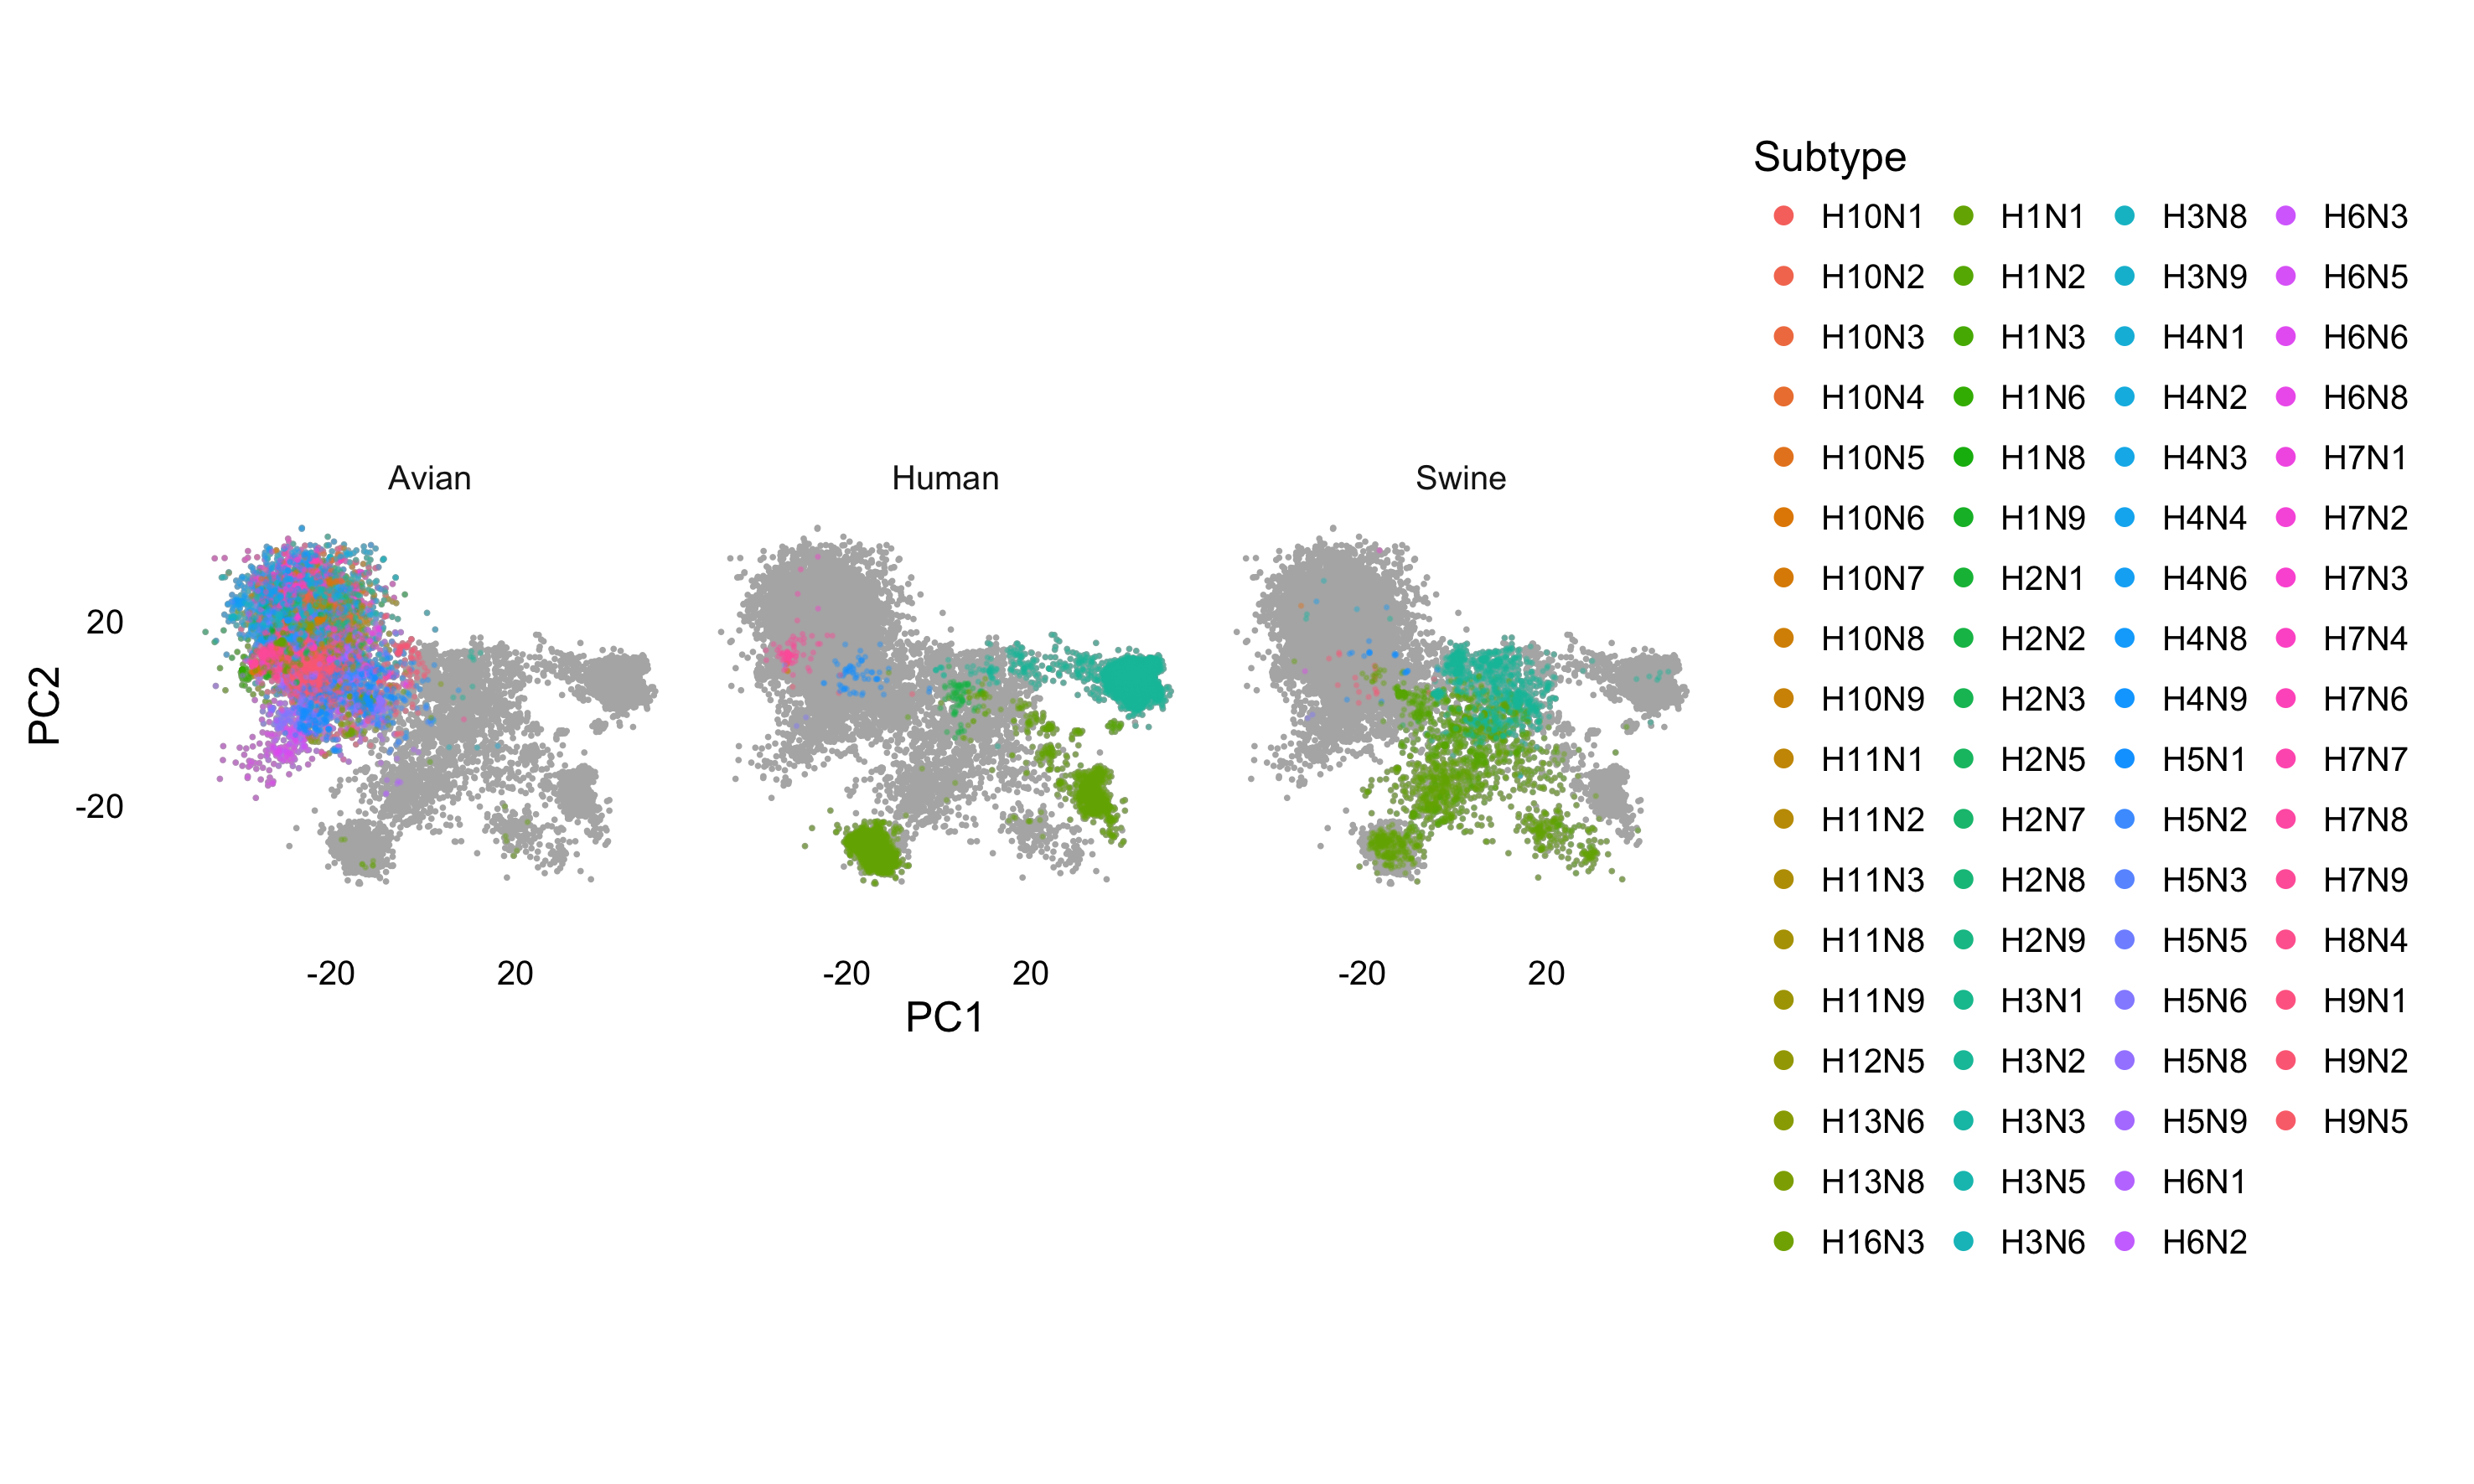
\includegraphics[scale=0.18]{pca_0dcec.png}\end{center}
    \caption[Subtype-specific clusters of codon usage via PCA.]{PCA of codon usage creates subtype specific clusters that are nested within larger host-specific clusters (compare Figure \ref{fig:pca1}). This is plausible because many subtypes prefer one host over another. Plot components are the same as in Figure \ref{fig:pca1}.}
    \label{fig:pca2}
\end{sidewaysfigure}


\subsubsection{Codon Usage Predicts Host Species with High Accuracy}

We fit an SVM based on IAV codon usage ($\hm{X}$) for 15k samples. This constitutes the balanced training set with 5k samples for each host (i.e. a stratified sample). Host labels (Avian, Human, Swine) were used as prediction target $\hm{y}$. This setup produced very good predictive results (Table \ref{tab:confusion-main} and \ref{tab:modeleval}): We could predict the correct host label for input sequences with an overall accuracy of 95\%. Our method's sensitivity (recall) was 99\% with an overall positive predictive value (precision) of about 92\%.


\begin{table}[htbp]
    \centering
    \begin{tabular}{c | c | c | c | c}
        $\hm{y}$ \textbackslash~$\hm{\hat{y}}$ & Avian & Human & Swine & All \\
        \hline
        Avian   & 3207  & 49    & 13    & 3269 \\
        Human   & 6     & 4470  & 82    & 4558 \\
        Swine   & 9     & 10    & 849   & 868  \\
        All     & 3222  & 4529  & 944   & 8695 \\
    \end{tabular}
    \caption[SVM classifier: Confusion matrix.]{Confusion matrix of the SVM classifier, where true $\hm{y}$ and predicted $\hm{\hat{y}}$ hosts are tabulated. For example, of a total of 3222 Avian samples, 3207 were correctly assigned to class Avian, while 6 and 9 were wrongly assigned to Human and Swine, respectively.}
    \label{tab:confusion-main}
\end{table}


% This table somehow causes compilation problems. Fix later if necessary.
\begin{table}[htbp]
    \centering
    \begin{tabular}{c | c | c | c | c}
        metric \textbackslash~host & Avian & Human & Swine &  All \\
        \hline
        accuracy & \phantom{} & \phantom{} & \phantom{} & 0.95 \\
        recall & 0.99 & 0.95 & 0.94 & \phantom{} \\
        precision & 0.88 & 1 & 0.89 & \phantom{} \\
        F1-score & 0.94 & 0.97 & 0.93 & \phantom{} \\
    \end{tabular}
    \caption[Model evaluation according to 4 standard metrics.]{Model evaluation according to 4 standard metrics. Overall, the SVM classifier is both very sensitive and specific.}
    \label{tab:modeleval}
\end{table}


We wanted to investigate what information the SVM actually used to make predictions, i.e. which aspects of the codon usage allow the separation of host classes. We refit the SVM to dinucleotide counts as well as to trinucleotide counts with an offset of 1 nt, so as to count trinucleotides but not codons. We restricted the analysis to the coding sequence of the HA protein because this sequence has the largest nucleotide entropy accross samples in the MSA (Figure \ref{fig:distribution-2nt}). We contrained the SVM to train on only 1k samples so that the resulting model generalizes better (i.e. is less prone to overfitting). As a side effect, the required computational load dropped substantially by about an order of magnitude.

As is to be expected, the performance of this model is not as good because we only used 1k samples during training (Table \ref{tab:confusion-3nt}). Interestingly, dinucleotide usage (Table \ref{tab:confusion-2nt}) is enough to assign the correct host in many cases, which is surprising, given that the distribution does not vary much between species (Figure \ref{fig:distribution-2nt}). Generally, separation between Avian an Mammalian classes does not seem to be a problem for the SVM, but distinguishing Human and Swine host species is.


\begin{table}[htbp]
    \centering
    \begin{tabular}{c | c | c | c | c}
        $\hm{y}$ \textbackslash~$\hm{\hat{y}}$ & Avian & Human & Swine & All \\
        \hline
        Avian   & 5524  & 227    & 576    & 6327 \\
        Human   & 168   & 11314    & 1251   & 12733 \\
        Swine   & 25    & 800     & 995   & 1820  \\
        All     & 5717  & 12341   & 2822   & 20880 \\
    \end{tabular}
    \caption{Model evaluation for codon usage.}
    \label{tab:confusion-3nt}
\end{table}


\begin{table}[htbp]
    \centering
    \begin{tabular}{c | c | c | c | c}
        $\hm{y}$ \textbackslash~$\hm{\hat{y}}$ & Avian & Human & Swine & All \\
        \hline
        Avian   & 4294  & 1048    & 985    & 6327 \\
        Human   & 173   & 8376    & 4184   & 12733 \\
        Swine   & 17    & 630     & 1173   & 1820  \\
        All     & 4484  & 10054   & 6342   & 20880 \\
    \end{tabular}
    \caption{Model evaluation for dinucleotide usage.}
    \label{tab:confusion-2nt}
\end{table}


\begin{table}[htbp]
    \centering
    \begin{tabular}{c | c | c | c | c}
        $\hm{y}$ \textbackslash~$\hm{\hat{y}}$ & Avian & Human & Swine & All \\
        \hline
        Avian   & 5519  & 408    & 400    & 6327 \\
        Human   & 201   & 6152    & 6380   & 12733 \\
        Swine   & 34    & 557     & 1229   & 1820  \\
        All     & 5754  & 7117   & 8009   & 20880 \\
    \end{tabular}
    \caption{Model evaluation for frameshift codon usage.}
    \label{tab:confusion-frameshift}
\end{table}


When we introduce a frameshift in the trinucleotide count (Table \ref{tab:confusion-frameshift}), we are no longer able to separate the human and swine classes. This is interesting because it means that codon bias is at least partly informative in the separation of host species, and it suggest a hierarchical model: The destinction between mammal and bird thus stems largely from k-mer frequency, but between closely related species such as human and swine, the SVM likely draws its information from codon bias.


\newpage\subsection{Analysis of Experimental Codon Bias}

Next we turned to an ML technique called \gls{gbt}. We chose this technique over SVM because the latter offer very little insight into why a particular classification was learned the way it was, i.e. SVMs are a rather black box. GBMs on the other hand are very transparent, because they are built from decision trees. These recursively split the data set: At each node of the split one can follow which decision was taken.


\subsubsection{Learning Host-Specific Loci Consistently using GBTs}

First, we wanted to verify that the GBT algorithm yields consistent results. From the \gls{iav} MSA we selected 100 positions at random to test this. With 2k one-hot encoded samples for each of the 3 host labels (Avian, Human, Swine) the resulting feature matrix had dimensionality $6(10^3) \times 400$. We ran predictions on a balanced test set of 1k samples for each host label. Then we repeated this process 20 times and logged the position-wise \gls{fi} score.

The resulting predictions are displayed in Figure \ref{fig:consistency} and are very consistent accross the 20 trials, i.e. the same positions are assigned approximately the same \gls{fi}. Random aspects of the GBT algorithm do not seem to cause different results when given the same input data.


\begin{figure}[H]
    \begin{center}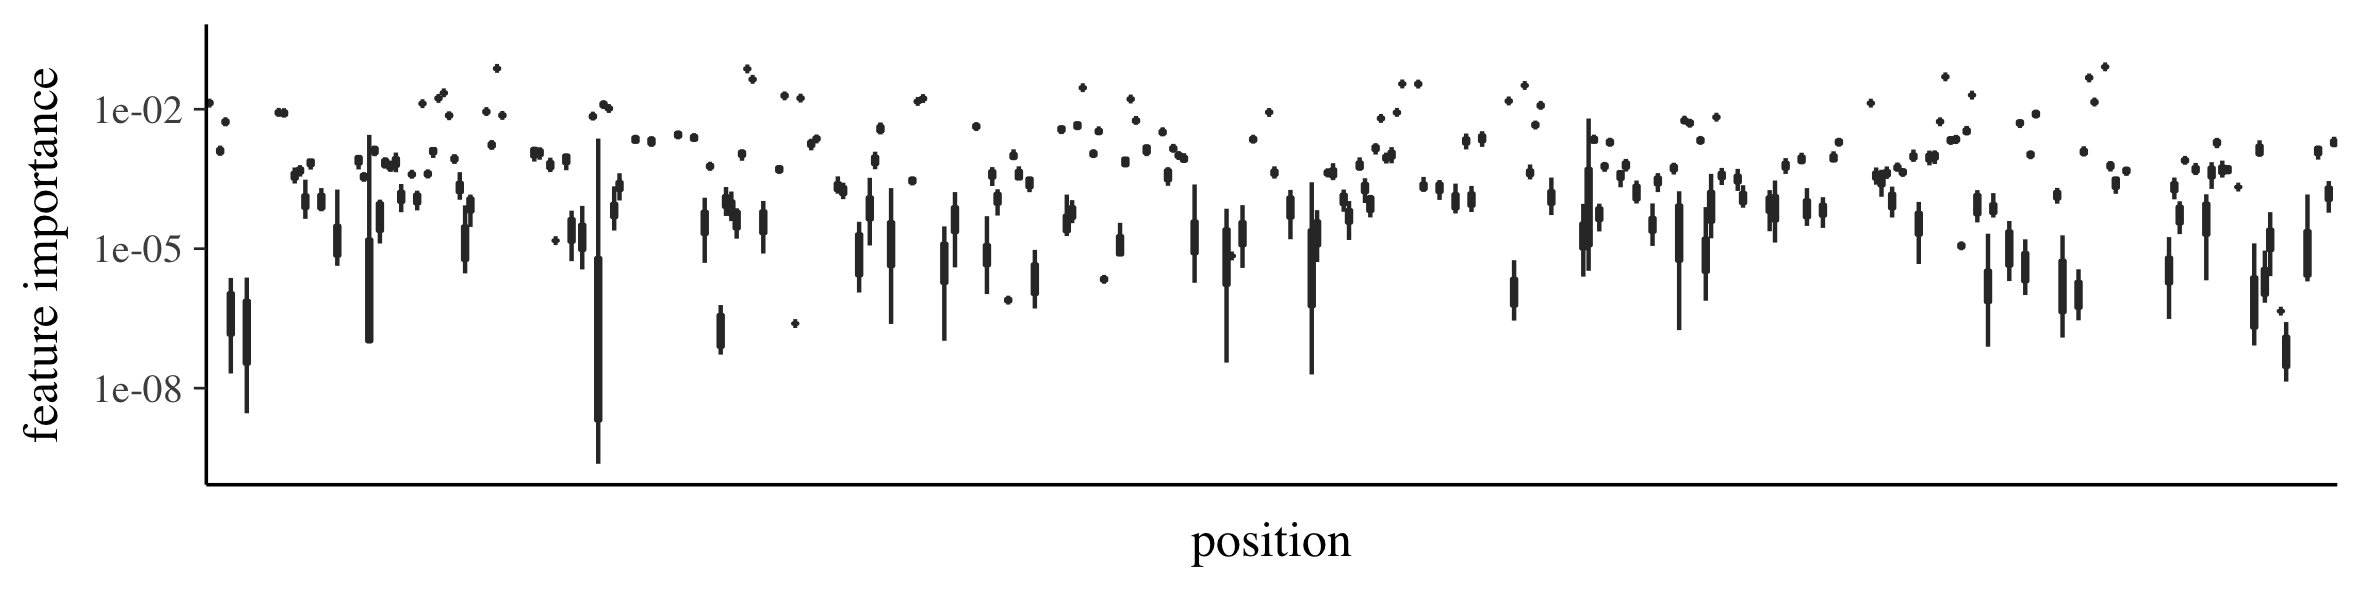
\includegraphics[scale=0.18]{PA_random100_repeat20_log.png}\end{center}
    \caption[GBTs assign consistent feature importances to tested loci.]{GBTs assign consistent feature importances to tested loci. The boxplot shows log feature importance on the y axis with loci being indexed on the x-axis. Note that because we one-hot encoded the nucleotide sequences, 4 positions in the index correspond to one position in the sequence. We observe very consistent learning behaviour from the GBTs with many irrelevant features being shrunken towards 0.}
    \label{fig:consistency}
\end{figure}


We then wondered whether the signal picked up by the GBTs is the entropy in each column of the MSA, i.e. the position-wise information. Figure \ref{fig:entropy-scatter} shows a scatter plot of the positional entropy along the PA gene of IAV. Note that while there seem to be 2 ``bands'' $y=\{0, 1\}$, the entropy distribution along the gene seems homogenous, i.e. we do not observe any entropy (i.e. mutational) hot spots.


\begin{figure}[H]
    \begin{center}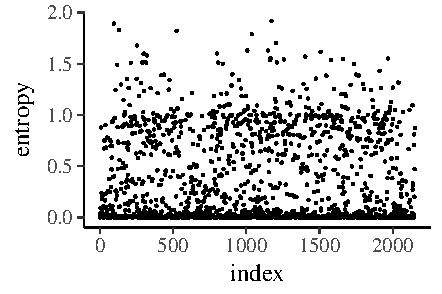
\includegraphics[scale=1]{entropy_PA_train_test.pdf}\end{center}
    \caption[Entropy of loci along PA segment.]{Entropy of loci (index) along PA segment. The entropy distribution along the PA gene seems homogenous without any obvious mutational hot spots.}
    \label{fig:entropy-scatter}
\end{figure}


The observed bands correspond to a bimodal entropy distribution with 2 modes around 0 and 1 (see Figure \ref{fig:entropy-freqpoly}). Note that when H = 0, all nucleotides at a particular locus are of the same type, i.e. the site is perfectly conserved.


\begin{figure}[H]
    \begin{center}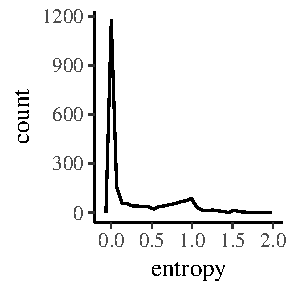
\includegraphics[scale=1]{entropy_PA_freqpoly.pdf}\end{center}
    \caption[Bimodal entropy distribution.]{We can observe a bimodal entropy distribution H. When H = 0 for a given locus, all sequences present the same nucleotide at this index. When H = 1, we observe only 2 nucleotides at this locus at a ratio of 1:1.}
    \label{fig:entropy-freqpoly}
\end{figure}


We then correlated entropy to feature importance for all loci with FI $> 5(10^{-4})$. We observed a roughly log-linear relationship (Figure \ref{fig:correlation}), although we did not quantify it. This relationship is plausible: a locus that is more informative from an information theoretic standpoint seems to be more important in the learning process.


\begin{figure}[H]
    \begin{center}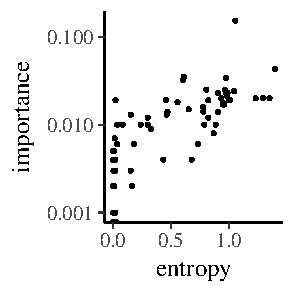
\includegraphics[scale=1]{entropy_PA_feat_importance.pdf}\end{center}
    \caption[Log linear relationship between entropy and feature importance.]{There is an approximate log-linear relationship between entropy and feature importance. Note however that we observe some loci which do not hold much information but nevertheless are important for classification. Those are likely host-specific minor variants, although we did not investigate this matter further.}
    \label{fig:correlation}
\end{figure}


Because entropy seemed very important for the predictive performance of the GBTs, we wanted to verify that the way we split our data set into a test and training sample (stratified) does not introduce an entropy bias. Figure \ref{fig:delta} confirms that this is not the case.


\begin{figure}[H]
    \begin{center}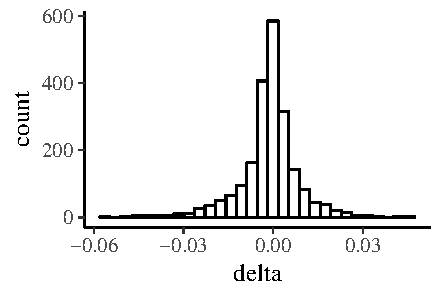
\includegraphics[scale=1]{entropy_PA_delta.pdf}\end{center}
    \caption[No entropy bias in test-train split.]{No entropy bias is present after the data set has been split into a test and training set. We calculated the position-wise difference between the test and training set and plotted the resulting histogram. Note how the entropy difference does not deviate substantially from 0.}
    \label{fig:delta}
\end{figure}


After these experiments we were confident that GBTs offered consistent performance on our learning problem. We next applied them to sequences that were subject to codon deoptimization.


\subsubsection{Inconsistent Feature Importance for Deoptimized Loci}

We analysed a total of 8 samples (including wild type) of Influenza virus A genomes that had been modified through strategies of codon deoptimization (Table \ref{tab:deopt-experiments}). The \gls{na} genes of IAV strain A/WSN/1933 (H1N1) were recoded (see methods section for protocol details). More specifically, the \gls{orf} was recoded between nucleotides 184-1200, such that 120 nt on both ends were left intact. Only non-terminal parts of the gene were targeted, because the 5'- and 3'- terminus sequences are important during IAV packaging: When the termini are deoptimized, no viable virions assembly fails (D. Kunec, personal communication).

To summarize Table \ref{tab:deopt-experiments}, the WT, DL, DM, HS, OG, and PD variants have the same codon bias (i.e. they contain the same codons) and are mainly distinguished by their \gls{cpb}. The H and HD have a different codon bias because they were designed with the aim of maximizing the GC content, where maximizing means iterative sequence changes up to a threshold above which no viable virions could be obtained.


\begin{table}[htbp]
    \centering
    \begin{tabularx}{\textwidth}{l | r | c | l | X}
        label & CPB & plaque size & name & description \\
        \hline
        WT & 0.004 & 1.00 & wild type & \\
        DL & -0.231 & 0.31 & deoptimized-less & codon pair deoptimized, less \\
        DM & -0.449 & 0.11 & deoptimized-more & codon pair deoptimized, more \\
        HS & -0.049 & 0.94 & high-score & same number of NNC-GNN codon pairs as in DM, and codon pair \\
        OG & -0.209 & 0.99 & optimized-good & same NNC-GNN codon pairs as in DM, and codon pair \\
        PD & -0.222 & 0.35 & pure deoptimization & same NNC-GNN codon pairs as in WT, and codon pair \\
        H & -0.207 & 0.52 & high & CpG maximized \\
        HD & -0.339 & 0.39 & high deoptimzed & CpG maximized and codon pair deoptimized \\
    \end{tabularx}
    \caption[Summary of deoptimized sequences.]{Summary of the deoptimization experiments. 7 deoptimized variants were constructed from 1 wild type IAV strain A/WSN/1933 (H1N1). CPB: codon pair bias, plaque size: a measure of virus viability/ attentuation (smaller means more attentuated).}
    \label{tab:deopt-experiments}
\end{table}


We then marked the deoptimized positions in a scatter plot of the previously learned feature importances (Figure \ref{fig:feature-importance}). We hypothesized that virus variants where \gls{na} loci of high \gls{fi} had been deoptimized would result in a more attenuated phenotype. However, no consistent signal could be observed: While some loci with high FI have been targeted by the deoptimization, we could observe no clear link between the FI of targeted loci and the resulting viability phenotype of the 7 IAV variants.

Note that the deoptimized sequences had already been designed with more or less heuristic principles before we started our investigation, so that our analysis was retrospective and did not inform the deoptimization targets priori.


\begin{SCfigure}
  \centering
  \caption[Deoptimized loci mapped to learned feature importances.]{Deoptimized loci mapped to learned feature importances for the ``DL'' variant (other variants not shown). The position-wise FI (light red) was learned from the above described host species prediction task using GBTs. We then superimposed the loci that had been subject to codon deoptimization (in dark red). While some loci with high FI have been targeted, we could observe no clear link between the FI of targeted loci and the resulting viability phenotype of the IAV variants (see plaque score in Figure \ref{tab:deopt-experiments}). FI is scaled by square root ($\sqrt{F}$) for easier visual inspection. Modified label 0: no, 1: yes, i: index. Note that the 4 facets \{A, C, T, G\} result from the one-hot encoding, where each sequence locus is transformed into 4 features. Each of those features could be informally translated as asking: ``Is a given nucleotide present at this locus?''.}
  \label{fig:feature-importance}
  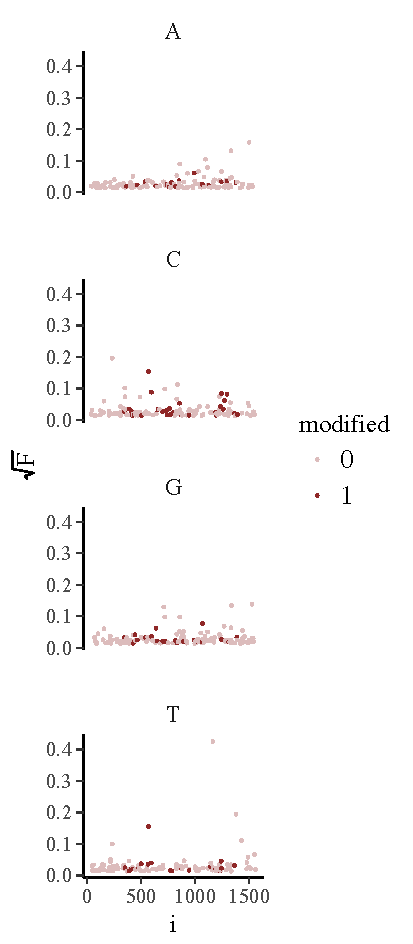
\includegraphics[scale=1]{NA_fi_deopt.pdf}
\end{SCfigure}


\begin{figure} % [H]
    \begin{center}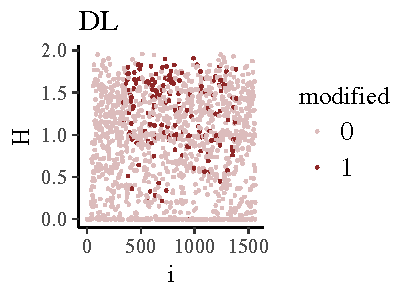
\includegraphics[scale=1]{NA_h_deopt.pdf}\end{center}
    \caption[Deoptimized loci marked in a scatter plot of entropy and index position.]{Deoptimized loci marked in a scatter plot of entropy and index position for DL variant of IAV. We can appreciate how only ``internal'' loci have been targeted by the deoptimization (color code as in Figure \ref{fig:feature-importance}). However, the deoptimization does not target high entropy loci specifically.}
    \label{fig:entropy}
\end{figure}


Similarly we did not observe a clear pattern concerning deoptimized loci with respect to entropy (Figure \ref{fig:entropy}).


\newpage


\subsection{zoo - A New Data Structure for the Exchange of (Viral) Data}

\begin{quotation}
\emph{Simplicity is a prerequisite for reliability.\\
-- E. Dijkstra}
\end{quotation}

\vspace{0.5cm}

\begin{quotation}
\emph{Equating simplicity with ease and familiarity is wrong.\\
-- R. Hickey}
\end{quotation}

\vspace{0.5cm}

The zoo software package is available at \hyperlink{https://github.com/viehwegerlib/zoo}{github.com/viehwegerlib/zoo} with detailed information on installation and usage as well as related background information in the form of a wiki. zoo can be cited under \colorbox{red-very-light}{\lstinline{doi.org/10.5281/zenodo.801560}}.

zoo is a tool to compose and manipulate units of sequence data in the form of so-called data cells, as well as a protocol to exchange them. Data cells are intended to be shared through a decentralized \gls{p2p} network, implementing an offline first design. A data cell's sequence content can be seached efficiently via Minhash signatures.


\subsubsection{Desiderata}

We pose three desiderata of a data structure in microbial bioinformatics:

First, it needs to have a rich data structure, e.g. allowing entries to be nested and/ or linked. This is necessary to represent biological data, which in spite of curative efforts remain mostly messy. The trend towards more entropy is likely to continue, while curative resources remain flat.

Second, the data structure needs a well designed \gls{api}, which allows complex queries. Ideally, it would also offer convenience functions to combine data in informative ways. For example, we would like to query sequence data by taxonomy as well as phylogeny. The API should link to downstream analyses with third party tools, e.g. for multiple sequence alignments and machine learning.

Third, we likely need to share data with collaborators and other stakeholders. Thus, the data structure needs to be implemented in a highly portable way, including easy and quick setup/ deletion as well as version control. The data structure is created for usage in the context of a project, and can be discarded after usage, while logging all the steps needed to recreate it if need be.


\subsubsection{An Atomic Unit of Data}

We termed the atomic unit of data in zoo a ``data cell''. We will leave definitions and implementation details for later and focus for now on a high-level description. A data cell is used to encapsulate the data in a sort of container and expose it to the outside world through a set of interfaces, which are provided by zoo.

zoo itself has two components: a (largely Python) library and a database engine. The engine stores and internally manages the data cell, and the library allows the user to work on the data through the interface.

Data cells can be composed like lego blocks. For example, a given curated data cell on flaviviruses can be updated with new experimental results. One could imagine such data cell composites to be directly attached to a publication, especially when a lot of new sequence data has been generated.


\subsubsection{The Data Cycle}

To use an abstraction, a data cell is a relay: Data from experiments or databases is distributed between collaborators and to and from downstream analyses (Figures \ref{fig:nz1} and \ref{fig:nz2}).


\begin{figure}[H]
    \begin{center}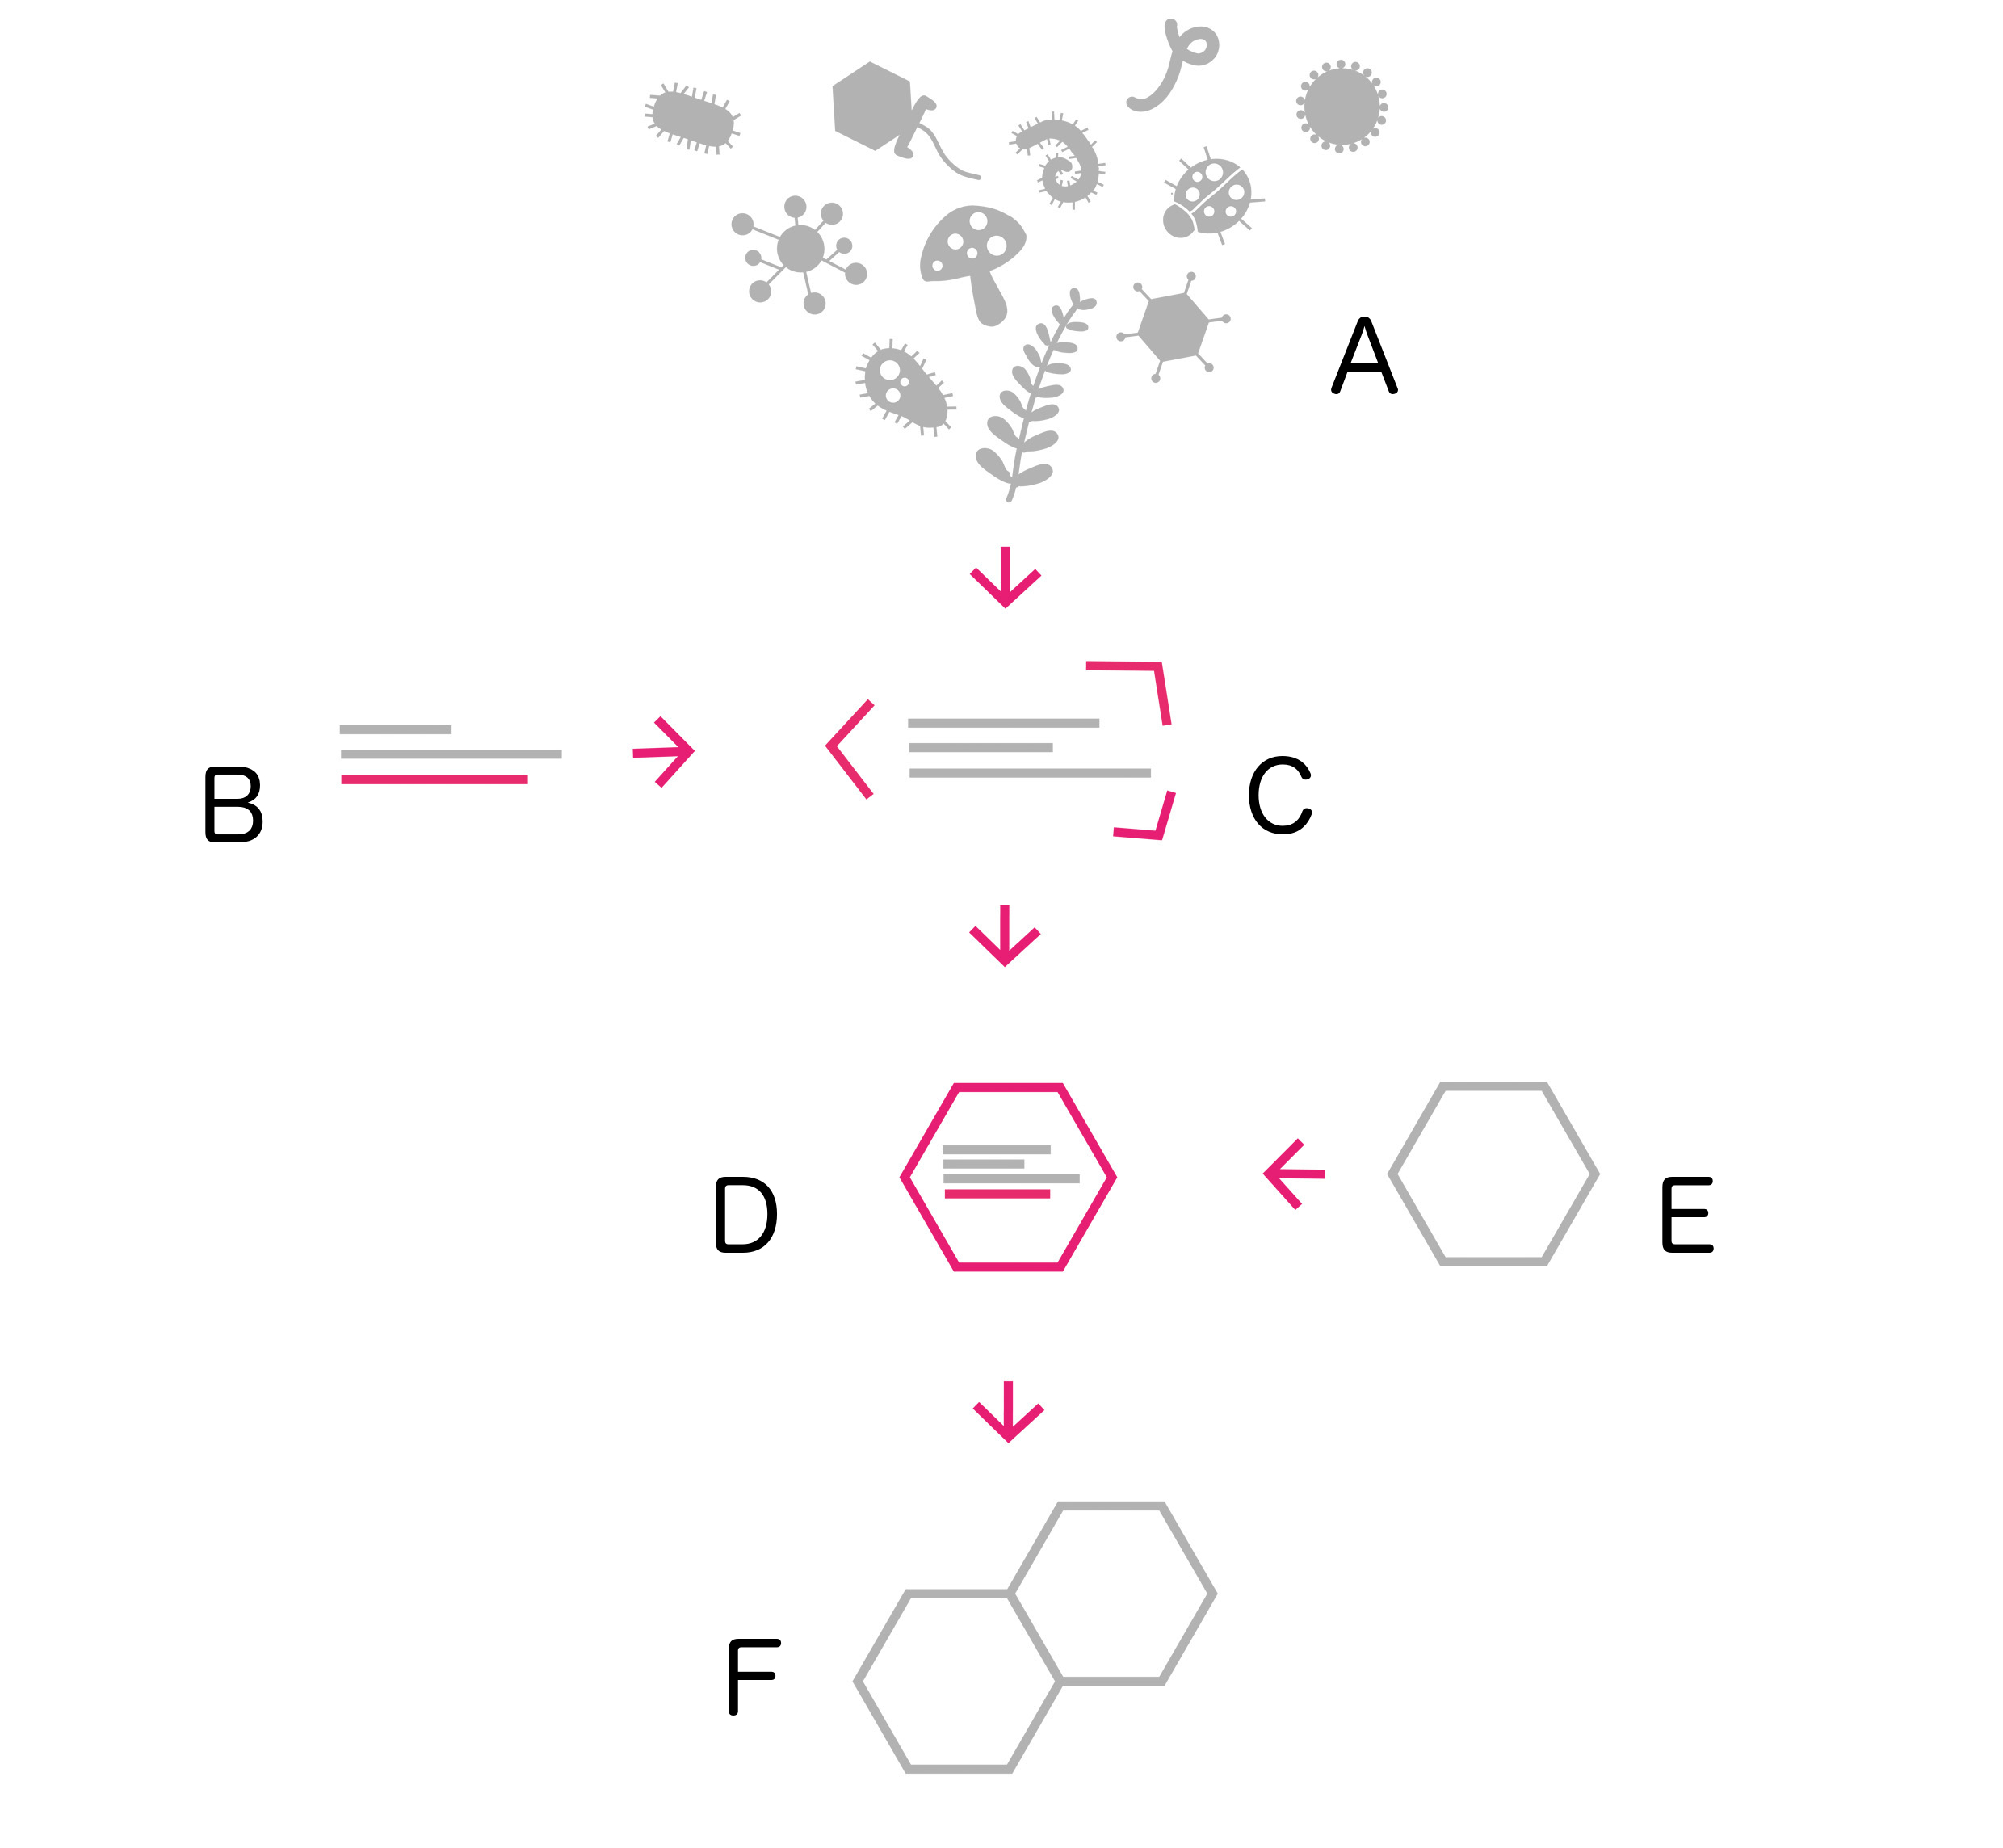
\includegraphics[scale=0.35]{nanozoo_broschuere_abwandlung_a4_part1_wletters.jpeg}\end{center}
    \caption[Infographic: Loading data into a data cell.]{Loading data into a data cell. Sample sequences - DNA, RNA or protein (A) - are combined with comparative sequences from databases (B) and ``containerized'' (C). This import process employs schemas to structure the data in predefined ways and to allow input validation. The whole construct is made accessible to the outside world through an interface. This process generates a data cell (D). Data cells can be composed with other data cells into composites (D + E = F), which implement the same set of interfaces and aim to be data backends that plug into downstream analyses (see Figure \ref{fig:nz2}).}
    \label{fig:nz1}
\end{figure}


By using the proposed protocol, data undergoes a sort of cycle (Figure \ref{fig:circle}).


\begin{figure}[H]
    \begin{center}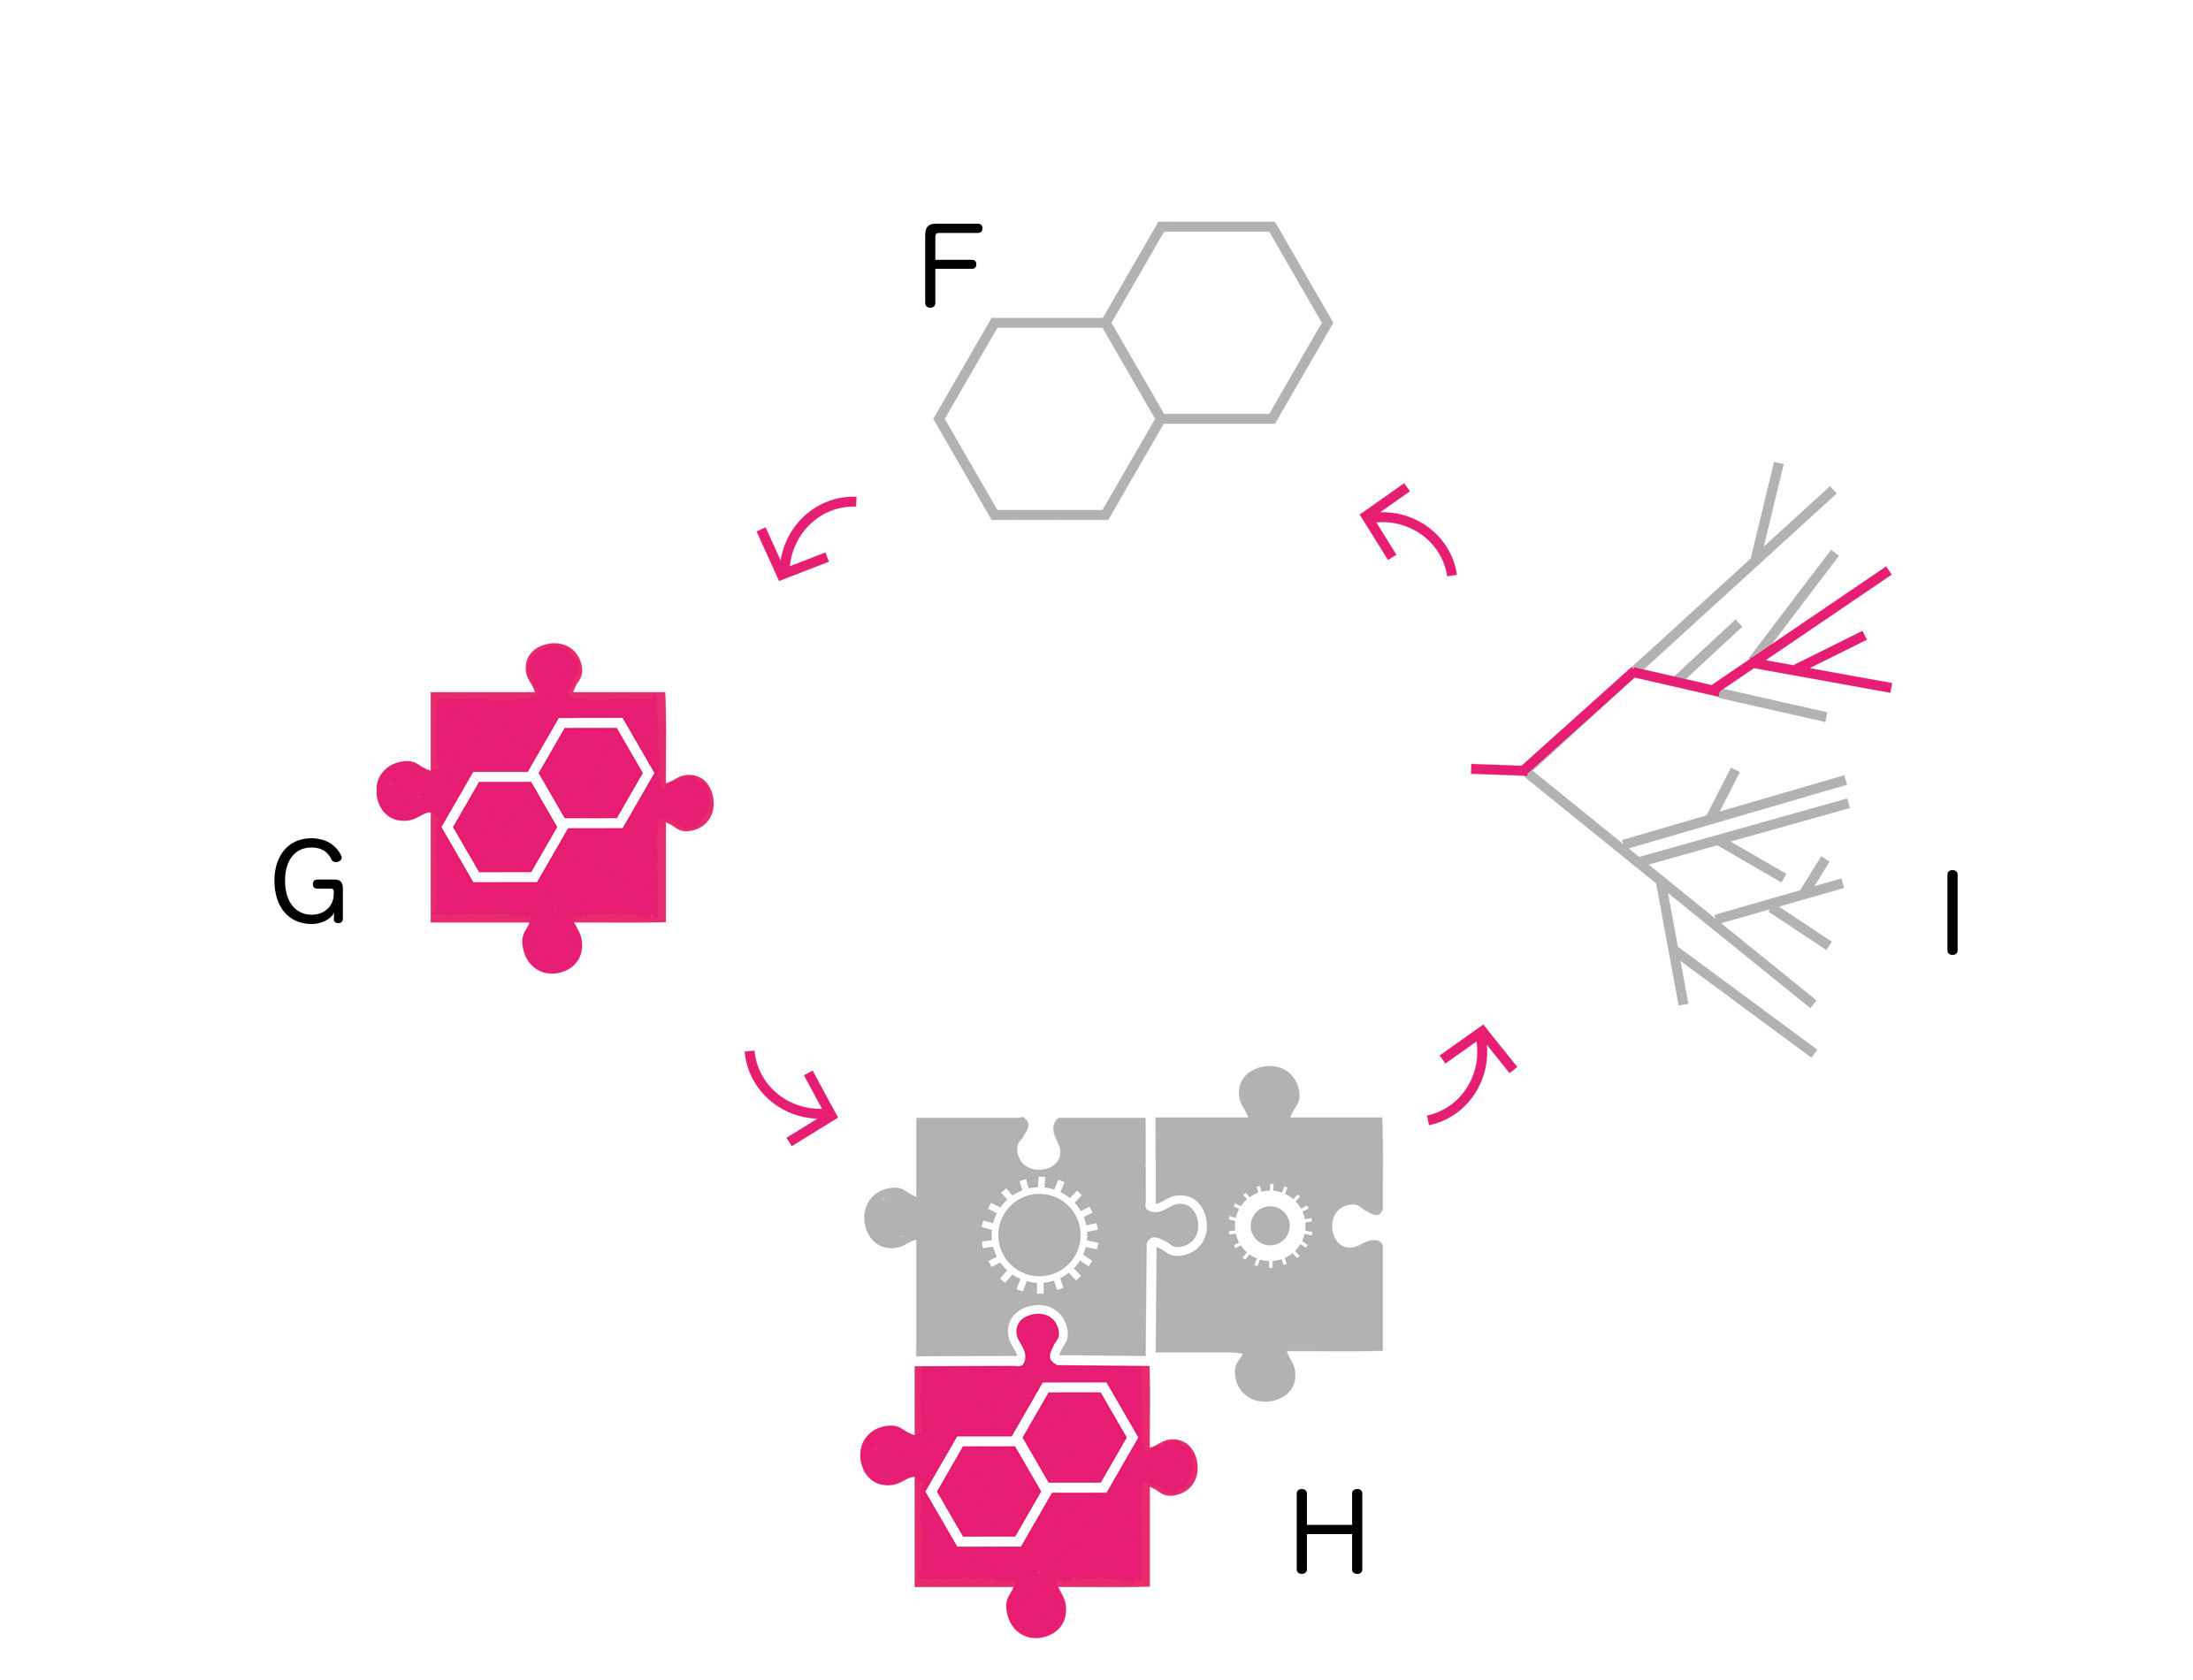
\includegraphics[scale=0.35]{nanozoo_broschuere_abwandlung_a4_part2_wletters.jpeg}\end{center}
    \caption[Infographic: Data cells are components that connect to downstream analysis pipelines.]{Data cells are components that connect to downstream analysis pipelines. A composite of data cells (F) can be plugged into downstream analyses (H) via zoo's API (G). Results from analyses such as sequence alignments or phylogenetic trees can be effectively stored in the data cell (I).}
    \label{fig:nz2}
\end{figure}


Raw sequence is annotated and analyzed with the analysis being integrated in the dataset. Consequentely, the more cyles a data set undergoes, the more curated is its content, and the more value is added to it.


\begin{figure}[H]
    \begin{center}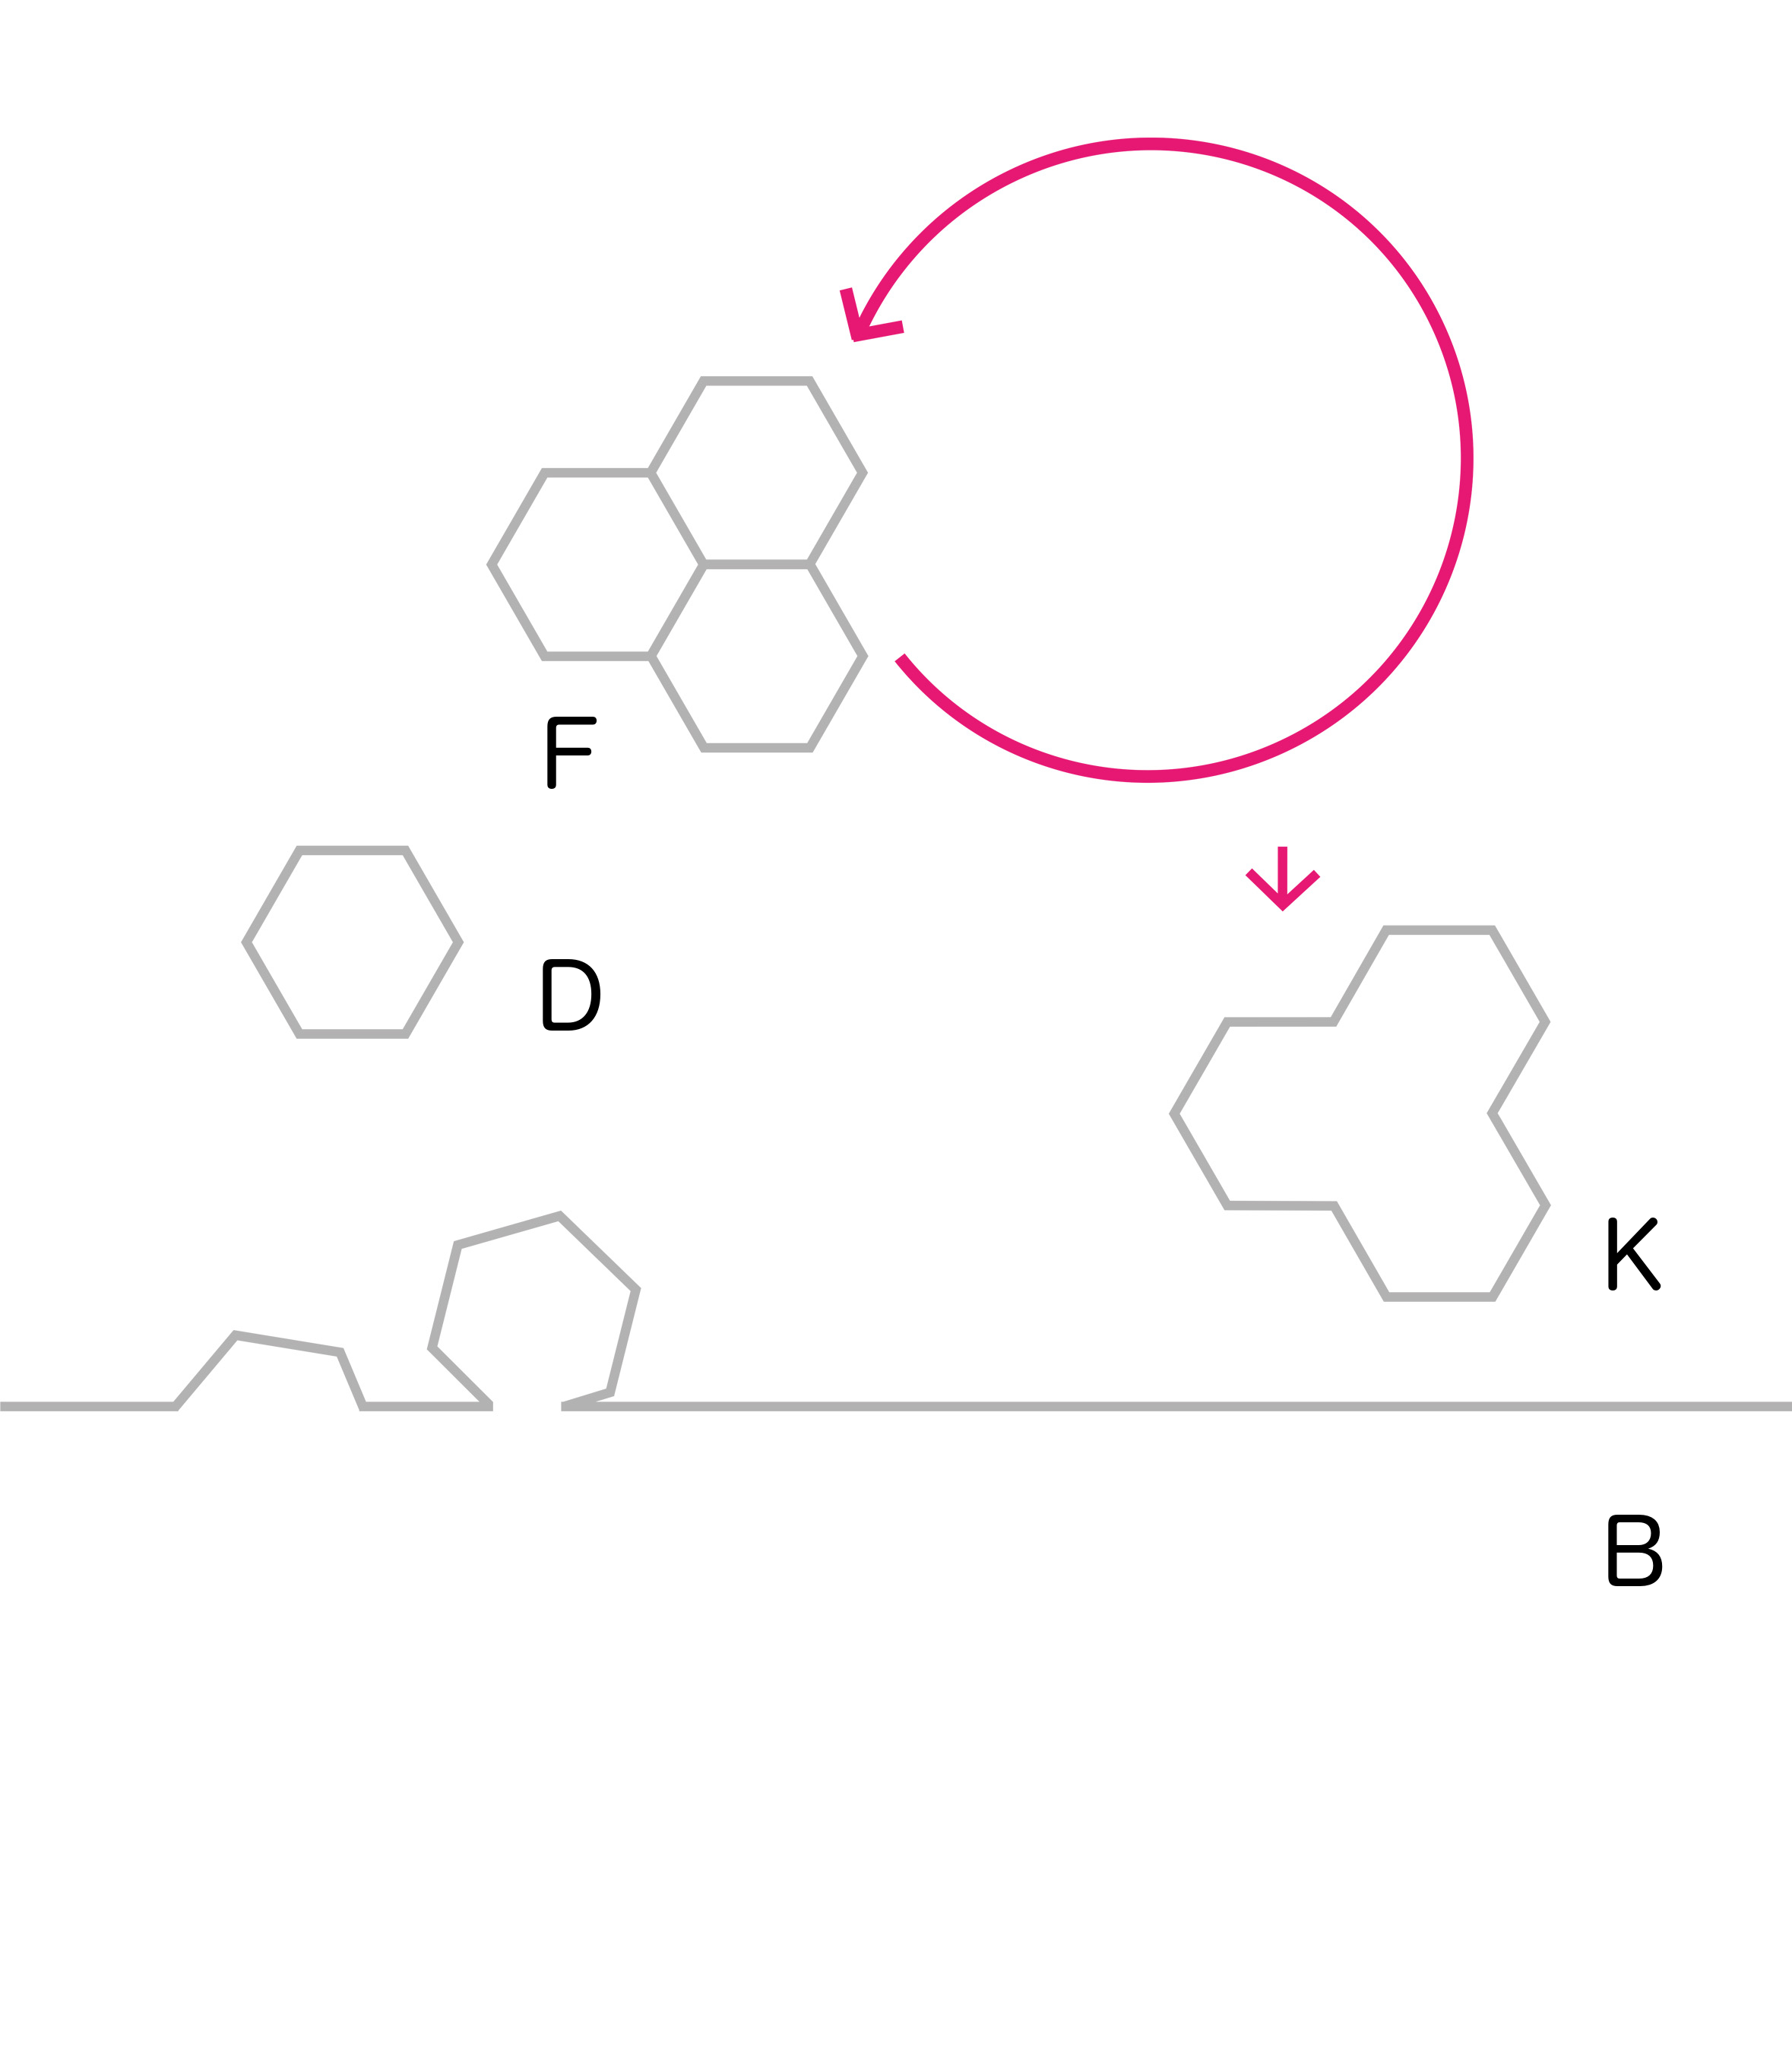
\includegraphics[scale=0.25]{nanozoo_broschuere_kreislauf_wletters.jpeg}\end{center}
    \caption[The data cycle.]{The data cycle. Data cells (D) ultimately constitute themselves in great part through public databases such as NCBI or EBI's ENA (B). They are then used as backends for analyses and store the results, which can be seen as a form of curation (F). After curation, the enhanced data is reintegrated into the public databases.}
    \label{fig:circle}
\end{figure}


From a more low-level perspective, zoo implements 4 activities on data: compose, manipulate, recycle and share.


\subsubsection{zoo: Compose}

A zoo database corresponds to a set of data cells. A data cell is a collection of documents (in NoSQL terminology). A document is a lightly structured nested hash map, typically transmitted in JSON format, a convention that zoo adopts as well. A document is composed of several schemas. These are predefined document components or templates, whose structure can be validated. For example, it can be checked whether an Influenza A virus document about to be inserted in a data cell has a correct strain nomenclature and whether a given segment is numbered from 1 to 8 or null. Because validation occures at the level of schemas, the whole database is valid by extension.

A small collection of schemas - both generic and specific to virus groups - can be found in the zoo documentation linked above. As an example, we specify here a full \gls{iav} schema composed of 5 schemas. For detailes documentation see \\ \hyperlink{https://github.com/viehwegerlib/zoo/tree/master/zoo/schema}{github.com/viehwegerlib/zoo/tree/master/zoo/schema}.


\begin{itemize}
    \item The minimum viable document in zoo is structured by a ``core'' schema with two fields (a field is a key: value pair): ``\_id'' and ``seq'' for identifier and sequence, respectively. The identifier is simply a primary key of the document. ``seq'' stands for sequence and is defined as a string with an arbitrary alphabet, typically RNA, DNA or protein. Although zoo was designed to work with microbes, especially viruses, it is agnostic to the origin of the sequence data, and as such can be used to model genomic complexities such as multiple isoforms and segmented genomes
    \item ``Metadata'' describe the way a sequence ``came to be known''. Where was it sampled from, who by, from which host, through which sample preparation and sequencing methods?
    \item The ``relative'' field includes taxonomic, phylogenic and linked information. It adresses how a given sequence compares to others. Alignments and phylogenetic trees are archived here.
    \item The ``derivative'' field summarizes or reexpresses the sequence information, e.g. via annotations, minhashes and alternative encodings like bracket-dot notation for secondary structures. Derived information is usually heavily dependent on the original sequence. For example, the annotation ``\gls{orf}'' derives from the sequence's start and a stop codon position.
    \item A (virus) specific schema, which in the case of IAV deals with some aspects of the genome structure (number and naming of segments) as well as nomenclature.
\end{itemize}

Note that all subschemas listed here are interacting: We could for example use Minhash signatures (derivative) to compare a sequence to other ones in the database, storing the result in a new field (relative).

Schemas can be composed. zoo implements a convenient notation to compose an arbitrary number of schemas in a nested document. For example, to nest metadata and annotation schemas in a core schema, we could write the following using zoo’s CLI:


\begin{lstlisting}[language=bash]
    zoo schema (core(metadata,annotation)) > schema.json
\end{lstlisting}


We can then validate records when we init/ add/ commit/ pull a data cell (see the zoo documentation for details), making sure they conform to the schema we specified earlier:


\begin{lstlisting}[language=bash]
    zoo init [...] --validate schema.json record.json
\end{lstlisting}


This makes for very flexible data entry. Instead of having a stiff format like a Genbank file we can construct hierarchical documents from prespecified components. Those are either adopted from the zoo repository or specified by the user.

On the side, this design addresses another issue: Because viruses are so diverse, it is difficult to specify a general schema that would do justice to all virus instances, past, present and future. With components, more general schemas like ``core'' and ``metadata'' can be composed with highly virus-specific ones, allowing a document to reflect nature instead of nature having to be coerced into a fixed document structure.

zoo offers many functions that facilitate work with nested hash maps, which is usually not provided out-of-the-box by many programming languages. See the docstrings of \colorbox{red-very-light}{\lstinline{zoo.utils.deep_set}} and \colorbox{red-very-light}{\lstinline{deep_get}} for examples.

zoo’s interface mostly encapsulates data. Within reason, it tries to expose data changes through common, standardized and tested operations, such as retrieving a sequence given annotation ranges. While zoo’s interface - i.e. its \gls{cli} and library (API) - handle schema composition and validation as well, its main value proposition lies in the activities of data manipulation, recycling and sharing.


\subsubsection{zoo: Manipulate}

From a practical viewpoint, working with virus data is tedious. That is not to say that people working with bacterial or human genomes are not to be pittied, but the sheer complexity and messiness of viral data is staggering. One of the problems is a lack of standardization, both in terms of taxonomy~\cite{Simmonds2017-sc, Calisher2016-mb, Simmonds2017-wj} as well as in terms of metadata. One usually has to assemble sequence data from various sources, complement annotations from another set of sources and hack together metadata based on incomplete records from a third set of sources. A tremendous amount of love and energy can flow into such curation. zoo assists with tools that make it bearable to structure data consistently in a document.

Because it runs on MongoDB, zoo supports complex queries of the form: \emph{All segments of virus X from 2007 onwards in a 500 km perimeter of Jena linked to Mosquito hosts, with sequences restricted to annotation Y and sequence similarity to some reference strain Z.} Furthermore, functions are implemented that allow the (stratified) sampling of documents based on metadata. Annotations can be quickly applied to the embedded sequence fields, and exported into a variety of formats. Furthermore, a larger part of the zoo library deals with the munging of data into e.g. binary feature matrices, which are directly compatible with standard machine learning and artificial intelligence libraries such as Scikit-learn~\cite{Pedregosa2011-yy}, Keras~\cite{Chollet2015-km} and Edwardlib~\cite{Tran2017-mc}. The overall aim is to minimize the time from input to analysis prototype.

For example, the creation of the following figure from data import to visualization took the author under 10 minutes to create. Note that the data had to be assembled from 4 different files in as many formats.


\begin{figure}[H]
    \begin{center}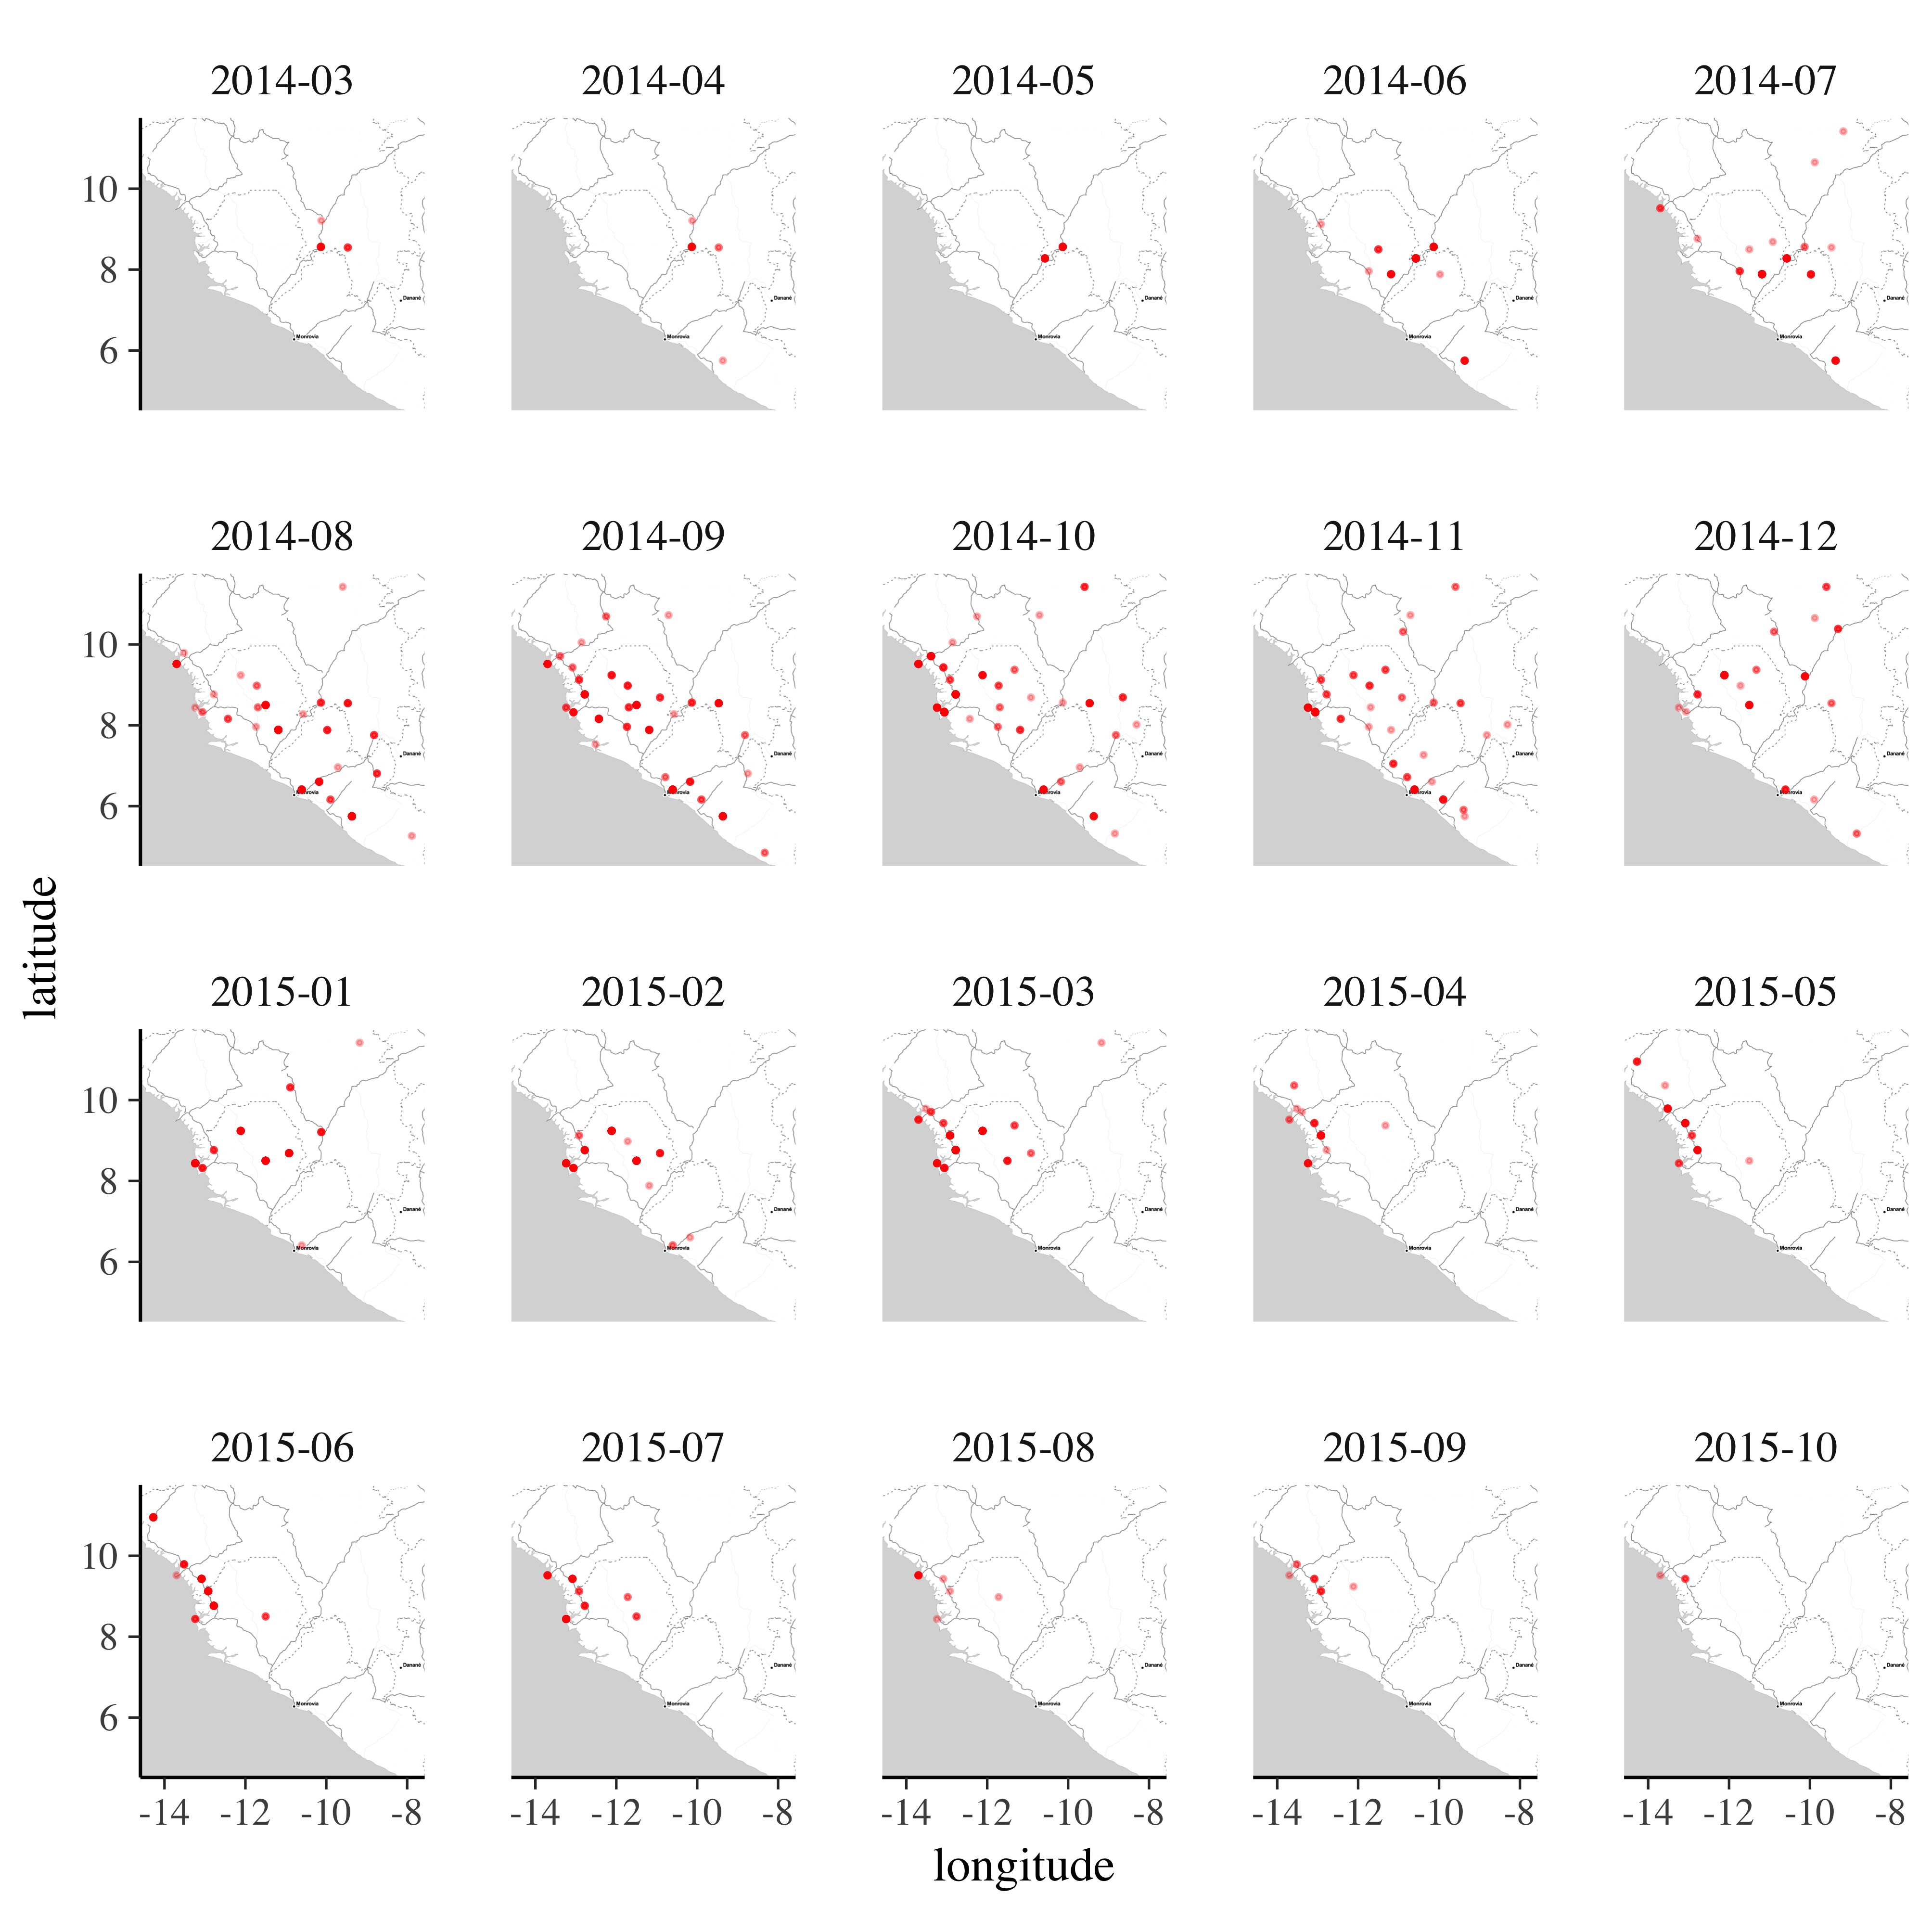
\includegraphics[scale=0.1]{makona.png}\end{center}
    \caption[Map illustrating the spatio-temporal progression of the Ebola epidemic.]{Map of the progression of the Ebola epidemic in small multiples (one for each month). Each red dot indicates a new case of Ebola. The map roughly spans West Africa, mainly Sierra Leone, Guinea and Liberia, where most Ebola cases of the outbreak 2014 - 2016 were located.}
    \label{fig:makona}
\end{figure}


\subsubsection{zoo: Recycle}

Running the same or slightly similar analysis more than once can be extremely wasteful. For example, if we computed an MSA already, it is not necessary to recompute it the moment we want to add another sequence. However, many times the first calculation is not available anymore or has a header that we slightly want to change the second time, and we end up recomputing everything. This is a wasteful practice.

zoo provides a set of functions under the title of ``digest'' (see the CLI documentation for \colorbox{red-very-light}{\lstinline{zoo digest [...]}}). They allow the decomposition of sequence alignments and tree structures into their constituents, which are then saved in the corresponding sequence’s document. For example, for an alignment an index of the loci where gaps have been inserted is stored under the ``relative'' field, together with a hash of the entire MSA. When we add new sequences to a data cell and want to extend the MSA with them, we simply reconstruct the initial MSA from the hash and gap index. We can freely modify the header format as well, because all the metadata is present in the document.

In the case of trees, zoo saves each leaf together with the path to the root in the corresponding sequence’s document. This is somewhat inefficient as we store internal nodes in many copies across multiple documents. However, we can then reconstruct the tree even though some documents might be missing.

Because zoo only works on data though its interfaces such as digest, the user is free to use whichever analysis programs she prefers. All that is required is that the output conform to standard bioinformatic formats that can be digested by and imported into zoo.


\subsubsection{zoo: Share}

zoo data cells are exported (``dumped'') to flat, human readible files in newline delimited JSON format, with one line per document. There is no prefixed header so this format is compatible with streaming applications.

These flat files are intended to be shared via \gls{p2p} networks such as Dat or IPFS, but are not limited to this. For axample, one could simple zip the dump and send it via FTP. P2P networks offer several desirable properties for information storage such as redundance, download speed and implicit version control, all of which have been adressed in the methods section.

Currently, data cells are primarily shared with the Dat protocol.


\subsubsection{Example}

To make the above explanations more concrete, we present an introductory code example that should illustrate some of zoo's command line functionalities.


\begin{minipage}{\linewidth}
\begin{lstlisting}[language=bash]

    # Create a JSON schema from zoo's templates to validate any data cell insertions.
    zoo schema (core(metadata(influenza),annotation)) \
    > schema.json
    # Or use your own.
    zoo schema --fp path/to/file (a(b,c)) > schema.json

    # Stream GenBank records to data cell, and validate schema.
    zoo load --source ncbi --fmt json \
    --ids accessions.txt --stdout - | \
    zoo init --db mockA --cell foo --validate schema.json -
    # ... Initializing data cell.
    # ... 42 entries inserted into cell "original".
    # ... Primary key assigned to field "_id".
    # ... inspect cell and commit

    zoo status --db mockA --cell foo --example

    # Make and commit changes (like you would with Git).
    zoo commit --db mockA --cell foo original
    # ... Dumping data cell.
    # ... Minhash signature computed for molecule type: DNA
    # ... | 42 Elapsed Time: 0:00:00
    # ... Done.
\end{lstlisting}
\end{minipage}


Sharing the created data cell is done over the Dat protocol. IPFS support is under development.


\begin{minipage}{\linewidth}
\begin{lstlisting}[language=bash]
    # share
    mkdir send
    cp original.json send/
    dat share send/
    # ... Syncing Dat Archive: .../send
    # ... Link:
    # dat://73401e1b931164763eccsomelonglinkcefc718ebf49f6b4fe4dbad7

    # In a faraway place, our collaborator (B) clones a copy of our
    cell and adds it to her "zoo" of other data cells.
    mkdir receive
    dat clone <link> receive/
    zoo add --db mockB --cell foo --primkey genbank.accession \ receive/original.json
    # ... Loading data cell.
    # ... Index created on field "genbank.accession".
    # ... 39 documents inserted in cell "foo".
    # ... 3 duplicates skipped.

    # Meanwhile, original.json was modified. B want his zoo to reflect
    # the changes:
    dat pull receive/
\end{lstlisting}
\end{minipage}


zoo supports commands known from the Git version control software, such as diff and pull.


\begin{minipage}{\linewidth}
\begin{lstlisting}[language=bash]
    # diff it
    zoo diff --db mockA --cell foo bar.json > diff.json
    # ... Searching for changes (delta).
    # ... Done.
    # We can pipe this, too.
    zoo diff --db mockA --cell foo bar.json | head -n2
    # Apply changes to data cell.
    zoo diff --patch --db mockA --cell foo diff.json
    # ... Loading and applying delta.
    # ... Done.

    # pull
    zoo pull --db mockB --cell foo receive/modified.json
    # ... Updating cell's md5 hashes.
    # ... / 0 Elapsed Time: 0:00:00
    # ...
    # ... 38 entries unchanged.
    # ... 4 entries replaced.

\end{lstlisting}
\end{minipage}


Two features other data structures do not offer is the reintegration of computed results with the ``digest'' command as well as support for probabilistic data structures (Minhash, SBT).


\begin{minipage}{\linewidth}
\begin{lstlisting}[language=bash]
    # Now put data cells into your favourite analysis workflow,
    # then use zoo's API to import/ export the results, like
    # multiple sequence or reference-based alignments, phylogenetic
    # trees, secondary structure ... happy exploratory
    # data analysis. Also, set global vars to reduce typing.
    ZOODB=mockB
    ZOOCELL=foo
    zoo digest --encode tree.nexus
    zoo digest --decode msa.mafft.fa

    # Not yet implemented: Send metadata about cell to a registry,
    # so others can discover it.
    zoo push ...

    # Create a sequence Bloom tree (SBT) from the minhash
    # signatures of a given cell.
    zoo sbt_index --db ref --cell virus --ksize 16 --nsketch \
    1000 virusref
    # ... Initialize SBT.
    # ... Compute minhash signatures for selected documents.
    # ... k-mer size: 16, sketch size: 1000
    # ... \ 9158 Elapsed Time: 0:01:45
    # ... Save SBT.
    # ... Done.

    # Use sourmash_lib to query other signatures about the
    # cell's SBT.
    sourmash sbt_search --ksize 16 virusref query.fa.sig
    # ... running sourmash subcommand: sbt_search
    # ... loaded query: survey.fa... (k=16, DNA)
    # ... 0.11 0ef85591-d464-4953-915f-f673907b7e8e
    # (here Zika reference genome)
\end{lstlisting}
\end{minipage}


Furthermore, zoo handles input and output in a way that is convenient and integrates well with UNIX pipelines (pipes etc.).


\begin{minipage}{\linewidth}
\begin{lstlisting}[language=bash]
    # Export, e.g. to fasta, JSON or stdout.
    zoo dump --query q.json --selection \
    _id,meta.date,meta.geo.cou,seq \
    --delim "|" --fmt fasta dump.fa

    zoo dump --query q.json --selection _id,seq \
    --fmt fasta - | head

    # Pipe into sourmash.
    zoo dump --query q.json --selection _id,seq --fmt fasta - | \
    sourmash compute -k 16 -n 100 --singleton --out q.sig -

    # Done, lets get some coffee.
    zoo drop --db mockB --cell foo --force
    zoo destroy --db mockB --force
\end{lstlisting}
\end{minipage}


\subsubsection{Scaling}

How does zoo scale? First, we need to think of what actually needs scaling, which are basically two things: The database size (including query speed) including the associated storage capacity as well as zoo’s core functionalities, such as Minhash.

A data cell can be moved to a larger compute environment if local resources are not sufficient anymore. Note however that we can load all available Influenza A virus sequences (> 700 k) from a Fasta file in less than 10 min, and query them in subsecond time on a typical laptop.

zoo's (database) engine is provided by MongoDB, the de-facto industry standard in NoSQL databases. MongoDB is known to be highly horizontally scalable to millions of documents. Cloud computing offers the required infrastructure, should the local capabilities run out. The P2P filesystem should not constitute a storage bottleneck, especially if financial incentives such as ``filecoin'' are introduced successfully.

One of the next milestones of zoo is to make the software available through a virtual machine container such as Docker or rkt. This makes the transfer to larger compute environments much easier.


\subsubsection{Integration of Minhash and SBT functions}

As described in to methods section, probabilistic data structures offer powerful ways to process large amounts of data partly with very limited resources.

In the case of zoo, the main value added comes from searching large sequence collections fast - albeit approximately - for similar sequences, and doing so in a streaming data paradigm. This can be employed as both a positive or negative filter. For example, if raw reads are queried against a data cell containing all known reference genomes (currently as of 2017 there are around 700k of them), we could filter out all known reads, and assemble only unknown ones, e.g. in the context of virus discovery. We can invert this too and use a data cell with genome variants of a single species to assign a query sequence to the closest strain, e.g. when assessing reassortment in Influenza A virus samples. With zoo it becomes trivial to set up these filters.

Also, the because all sequences are unsymmetrically hashed before we query them, this paradigm can be used with sensitive data where privacy considerations are important. For example, when a data cell is committed and a metadata registry entry prepared together with the sequence minhash, the same dataset can be queried without the person on  the other end having access to the raw sequence data. In a way, zoo provides a BLAST-like search experience of the registry, without providing access to the underlying raw data, which is handled by the user herself.
